\documentclass[11pt]{article}              % Book class in 11 points

\usepackage[ruled]{algorithm}
\usepackage{algpseudocode}

\usepackage{amsmath}
\usepackage{graphicx}
\usepackage{todonotes}
\usepackage{tabularx}
\usepackage{latexsym}    
\usepackage[ruled]{algorithm}
\usepackage{algpseudocode}
\usepackage{acronym}
\newcommand{\quotes}[1]{``#1''}
\usepackage{csquotes}



\parindent0pt  \parskip10pt             % make block paragraphs
\raggedright                            % do not right justify

\title{Autonomous Vehicle Plan Execution and Verification: 2015-2016 Report}   % Supply information
\author{Matthew O'Kelly, Houssam Abbas, Aditya Pinapala, Rahul Mangharam \\ \large University of Pennsylvania,
	Philadelphia, PA, U.S.A.\\}              %   for the title page. 
\date{\today}                           %   Use current date. 

% Note that book class by default is formatted to be printed back-to-back.
\begin{document}                        % End of preamble, start of text.

\begin{figure}
	\centering
	
\includegraphics[scale=0.25]{figures/apexlogo}
\end{figure}

\maketitle                              % Print title page.

\pagebreak
\section*{Executive Summary}
\pagebreak
\tableofcontents                        % Print table of contents
\pagebreak
\part{Background}
\section{Introduction}
 \subsection{Software agents are now drivers...}
The NHSTA describes Level 4 autonomous vehicles as designed:
\begin{displayquote}
	\emph{To perform all safety-critical driving functions and monitor roadway conditions for an entire trip. Such a design anticipates that the driver will provide destination or navigation input, but is not expected to be available for control at any time during the trip. This includes both occupied and unoccupied vehicles. By design, safe operation rests solely on the automated vehicle system.} 
\end{displayquote}

In a letter to \emph{Google Inc.} regarding their Level 4 autonomous vehicles, the NHSTA states:
\begin{displayquote}
	\emph{Once the AV is determined to be the driver for purposes of a particular standard or test, the next question whether and how Google could certify that the SDS meets a standard developed and designed to apply to a human driver. In order for the NHSTA to interpret a standard as allowing certification of compliance by a vehicle manufacturer, NHSTA must first have a test procedure or other means of verifying such compliance.}
\end{displayquote}

Given this interpretation of the latest AV technology, and the ever-growing gap between the capabilities of current testing frameworks and regulations several pressing questions \emph{must} be answered:
\begin{itemize}
	\item The NHTSA states AV software is considered a driver. How does one bound the risk posed to society by an autonomous software agent?
	\item A driver's license is a set of tests, we attempt to generalize human behavior based on tests. AV's don't necessarily fail in predictable ways. Tests cover an infinitesimal portion of the state space. How do we gain confidence that algorithms are sound, free of bugs, or even ethical?
\end{itemize}

Our perspective encompasses an integrated approach that captures the manifestation of errors in the physical world. At its heart is the use of formal models of system and precise mathematical specifications of desired behavior. Specifically in APEX, we are interested in developing the appropriate formal models, a set of specifications, and a battery of testable scenarios. As part of this work we must investigate how such methods scale, or fail to scale, and provide new solutions and interfaces to the underlying tools. 
 
 \subsection{How do you give a self-driving car a driver's license?}
 Each year there are an average of 1.24 million traffic fatalities around the world \cite{Waldrop2015}. Estimates indicate that more than 90 percent of all accidents are due to driver error \cite{Waldrop2015}. Competent autonomous vehicles (AVs) could drastically reduce the occurrence of such incidents, but a major question first needs be answered:
 how can we judge when an AV is ready to graduate from research laboratories to public roads?
 One thing is clear: the public will want significant evidence that AVs are indeed safe \cite{weld1994first}. 
 This raises significant ethical and legal questions about how the AV should behave, and technical questions about how to \emph{verify} that it will always behave the way its designers intended.
 
 Prototype AVs have driven millions of miles and are even being approved for \emph{testing} on public roads in some states \cite{Iozzio2014}; however, manufacturers cannot \emph{verify} (i.e., guarantee) the safety of even the simplest of scenarios in the presence of other dynamic traffic participants. 
 Compounding the difficultly of vehicle certification, vehicle manufacturers such as Tesla are transitioning to frequent over-the-air software updates. Such practice eschews conventional vehicle development technique and greatly increases pressure on developers to deliver correct software at a rapid pace. 
 
 The net result is a wide gap between current regulations and our technological capabilities. 
 Human drivers are not `certified' to act safely in all situations, in fact, we know they don't; however, they assume liability for their actions.
 Who is liable for the behavior of an AV? The manufacturer or the vehicle owner?
 Currently, it appears that manufacturers will take one of two approaches: (1) assume liability for the actions of the vehicle and self-insure \cite{volvo15Liability} or (2) force the human occupants of an AV to make all critical decisions and shift liability to the pilot \cite{maurer2015autonomes}. In either case, even if AVs reduce accidents by 99 percent, it is likely that the 1 percent of remaining accidents will invariably spawn a myriad of legal actions against \emph{both} manufacturers \cite{russell2015research} and vehicle owners.   
 If the legal question is not answered, these risks could stifle the development of the AV market.
 
 Thus, regardless of where legal liability falls it is clear that we first need new, practical methods for verification and validation of the decision engines of each AV.
 Furthermore, verification must be automatic, exhaustive, and expedient for clearly defined scenarios. 
 Secondly, ethical considerations still underlie both the design and verification of AVs: how does the safety of the car's passengers weigh against that of people in its environment? 
 Whose morals are embedded in the decision engines of an AV?
 
 \subsection{New and Old Challenges}
 
 Some of the problems facing would-be AV manufacturers in 2016 are very similar to those outlined by the teams in the DARPA Urban Challenge \cite{buehler2009darpa}. One problem highlighted by the first ever crash between AVs at the Urban Challenge \cite{fletcher2008cornell} is that there are no known \quotes{formal methods that would allow definitive statements about the completeness or correctness of a vehicle interacting with a static environment, much less a dynamic one} \cite{urmson2008autonomous}.  Today one must still consider the massive configuration space of each individual snapshot of the day-to-day life of an AV if verification is to be attempted. For example, in order to test the interaction between two 7 DOF AVs requires $10^{14}$ simulations for only 10 samples from each state. If each test takes 10 seconds, the resulting set of simulations will take \emph{30 million years} to complete. Furthermore, within a given scenario, errors in localization, sensing, and actuation imply we never know the state of the world exactly. Small state estimation errors can befuddle motion planning algorithms and mean a difference between collision and safety in tight spots. As many teams in the Urban Challenge noted, a means of verifying the safety of autonomous driving is paramount to putting self-driving cars in the hands of the public \cite{urmson2008autonomous}. 
 
 In contrast to the Urban Challenge in 2007, in which only 6 teams out of an original 89 applicants were able to finish, many research labs find themselves in the position of being able to construct a convincing AV in a matter of months; such a vehicle might be relatively competent in 75 percent of the situations it faces, but the long tail of special cases beckons. In fact Sebastian Thrun, a veteran of Google's Self Driving Car project and the Urban Challenge, notes that \emph{there were many more of unusual situations than we believed in the beginning}. One possible solution to handling rare events and scenarios is to record such occurrences using consumer vehicles driving in real traffic; with each new scenario existing behavioral planners can be adjusted via a reinforcement learning scheme \cite{wei2013autonomous, Silver_2010, Waldrop2015}. Just as in the more vanilla scenarios, timely updates to controllers provided on the basis of a single example will need to be verified offline, before shipping, and without the thousands of miles of testing necessary for a typical safety feature. 
 
 \begin{figure}
 	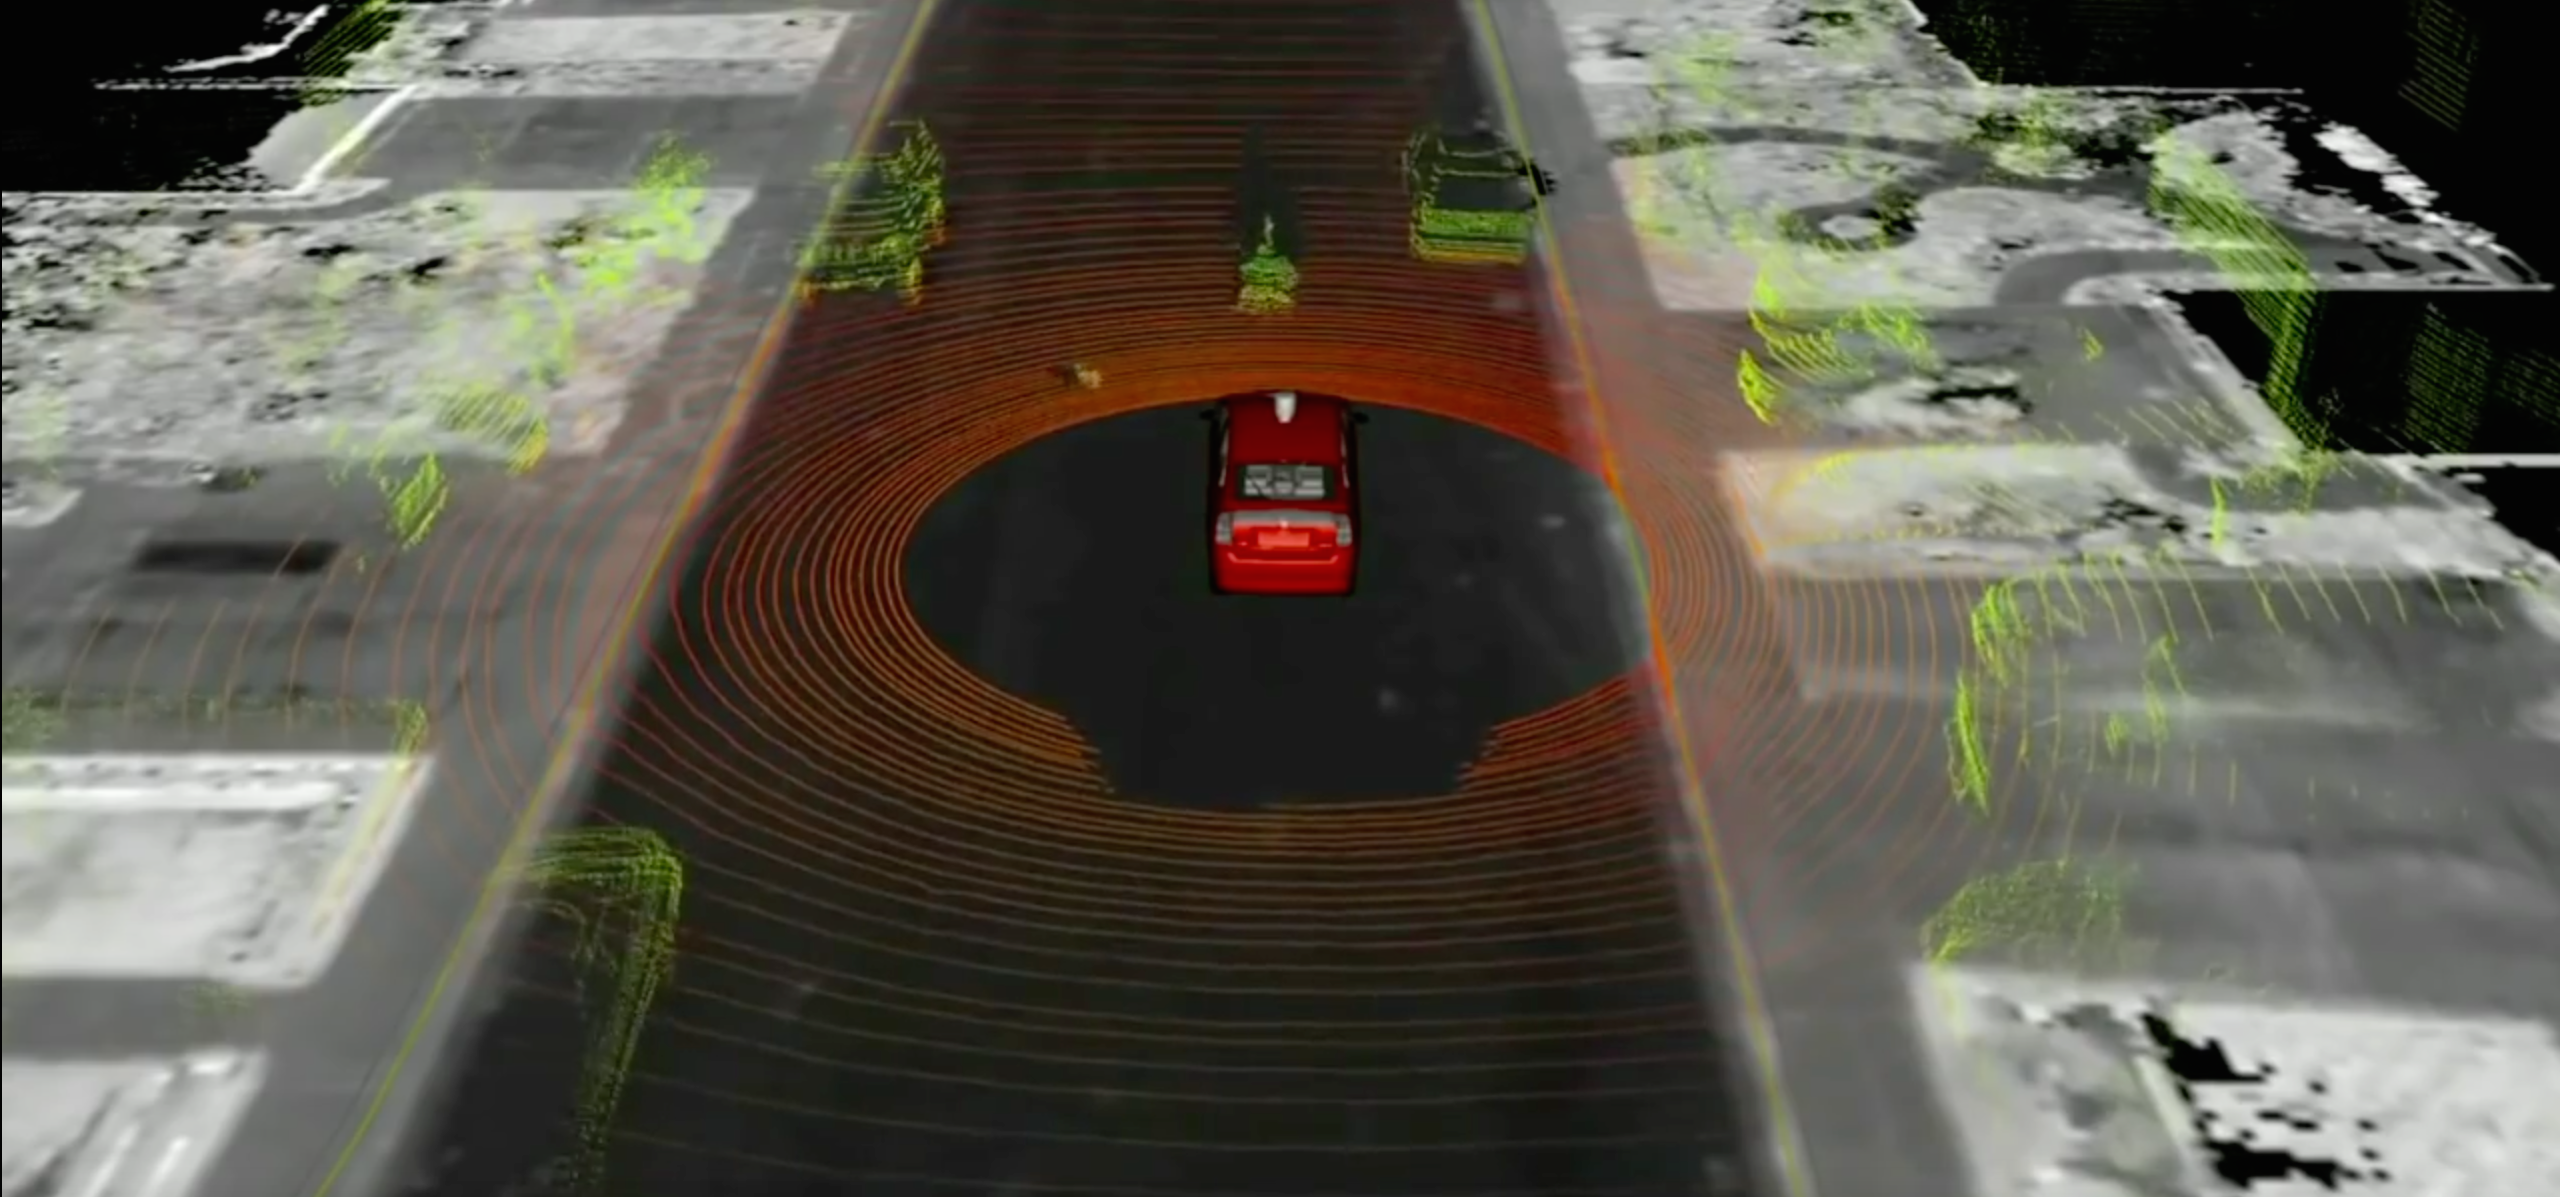
\includegraphics[width=\columnwidth]{figures/duck.png}
 	\caption{New Challenges: A woman in a wheelchair chasing a duck; autonomous vehicles are driving in real traffic engineers face an extremely long tail of events for which they must provide solutions}
 \end{figure}
 
 
 %As Brian Soublet of the California DMV pointed out, he knows how to test a 16-year-old's driving skills, but he can't say the same for a car. At the same time, these regulators know that when a death inevitably happens—no amount of %self-driving cars will reduce annual road deaths to zero—they'll be attacked for allowing unsafe vehicles on the road.
 
 
 \subsection{The APEX approach}
 The APEX tool represents a new approach to solving both the problems of the Urban Challenge and investigating rare events encountered only through on road driving and testing. Unlike other tools capable of verifying controllers for hybrid systems we require almost no abstraction. Most current approaches look at only the behavioral layer and assume perfect implementation of plans at the motion planning layer. Instead, we propose that the behavioral layer is used to generate sequences of problems to be investigated at the level of motion planning and trajectory tracking.  Thus, APEX addresses the safety verification issue by leveraging new results in hybrid systems and reachability analysis \cite{gao2013satisfiability} to convert a brute force search over real intervals (which is intractable) into a set of finite sequences of bounded reachability problems. 
 \begin{figure}
 	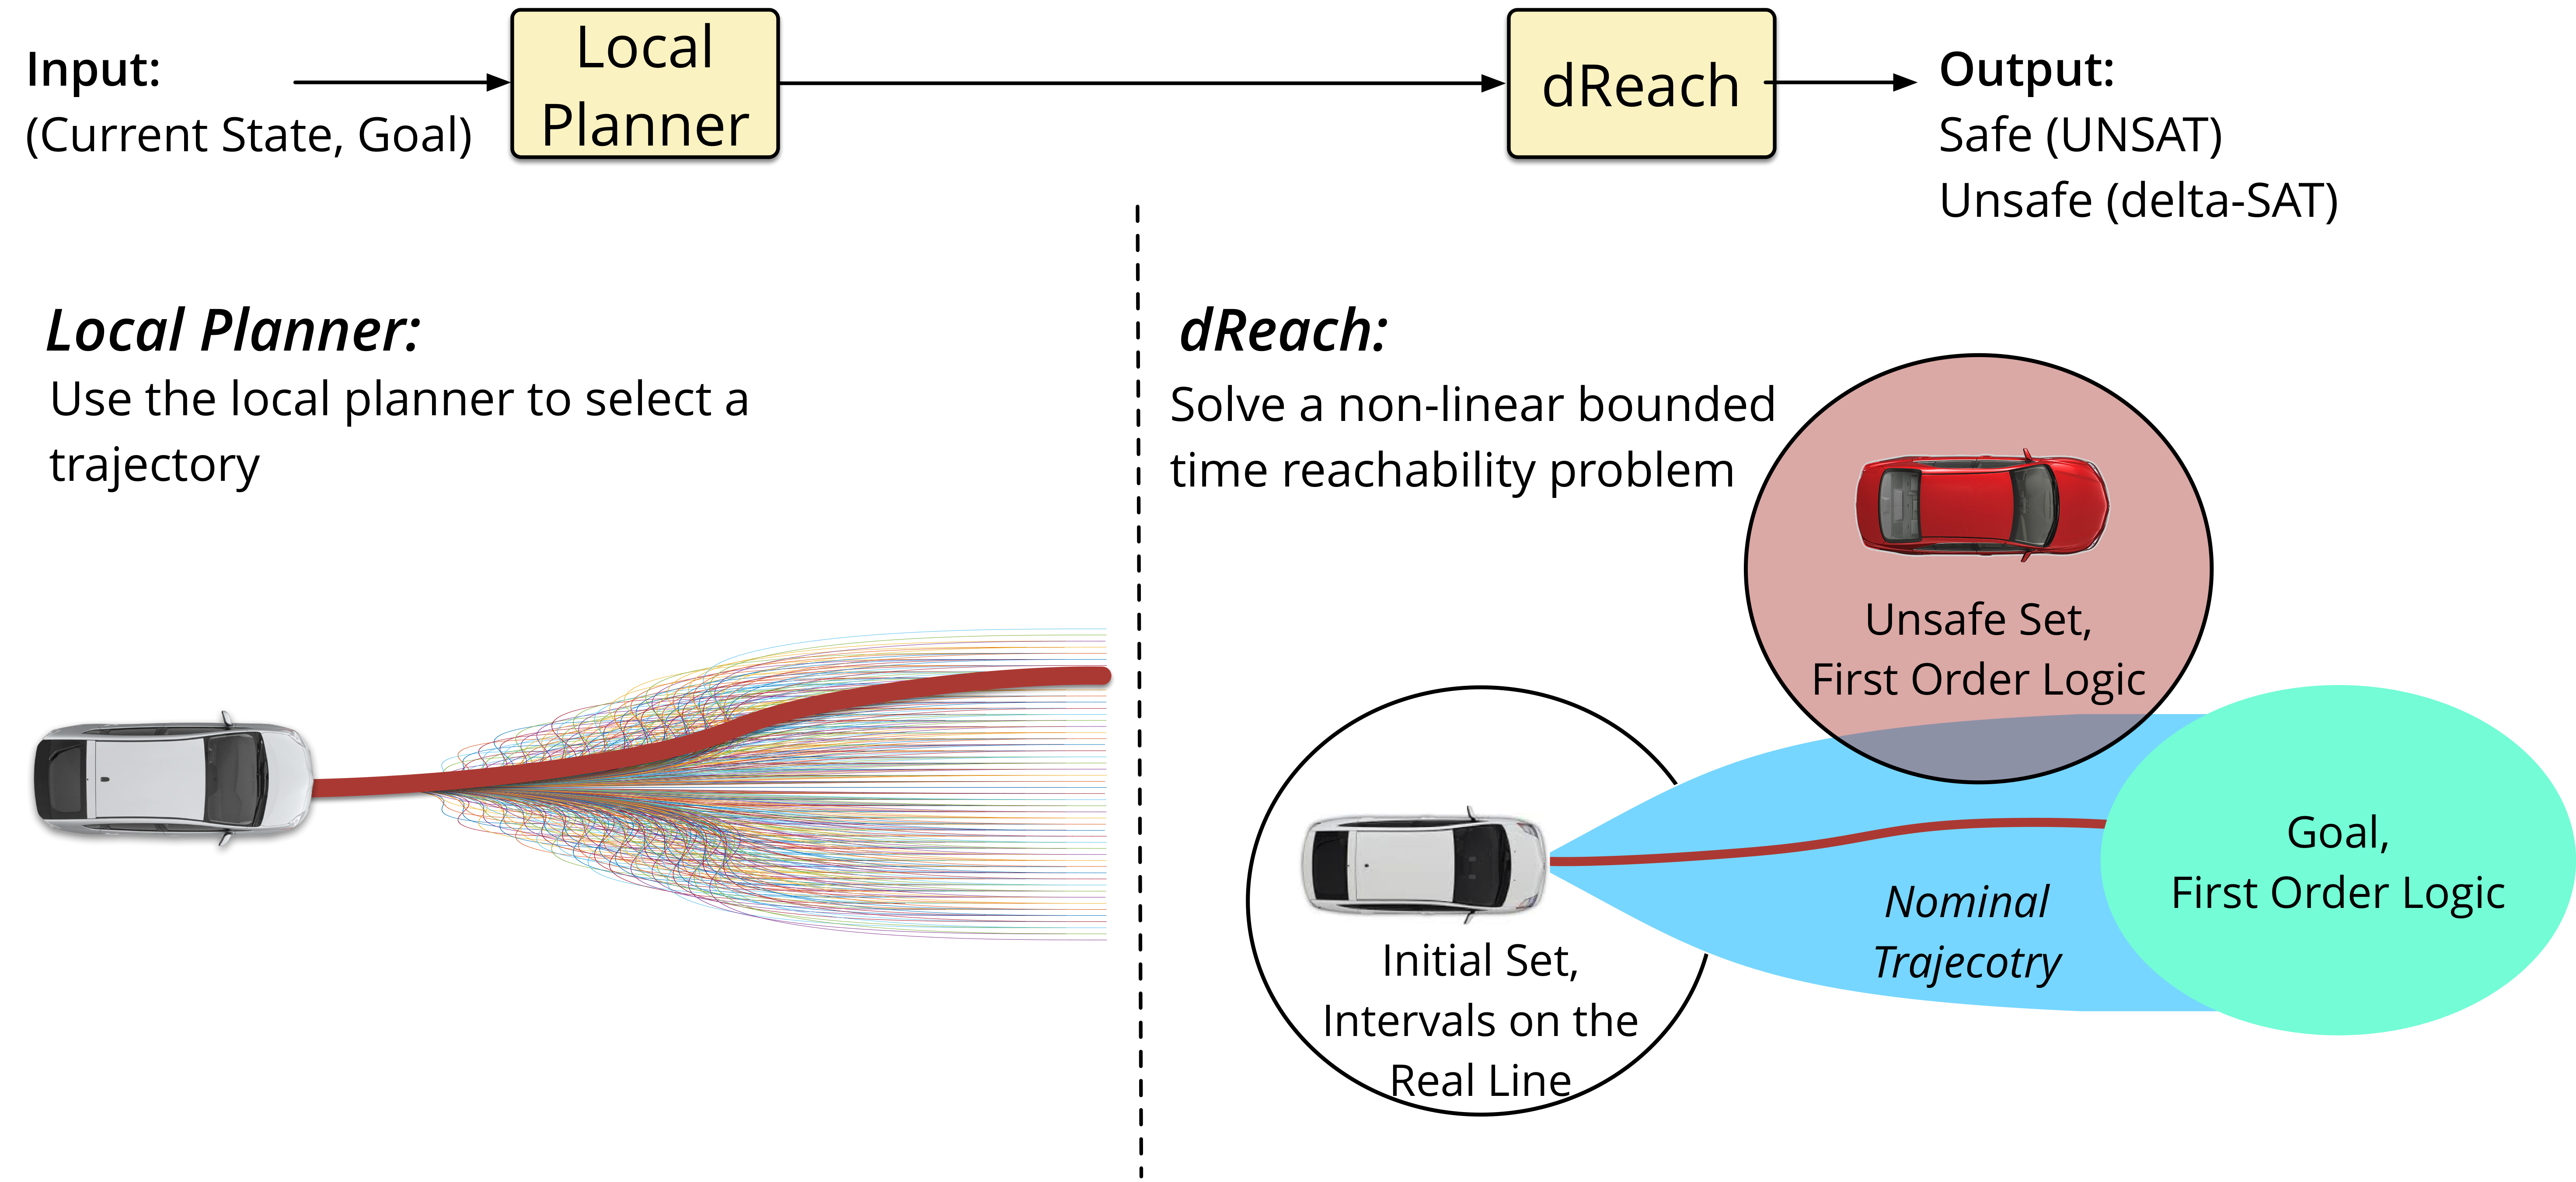
\includegraphics[width=\columnwidth]{Figures/tool_single}
 	\caption{A single offline execution of the APEX tool calls the local planner associated with the AV in order to generate a reachability problem}
 \end{figure}
 
 Using APEX we capture the output of trajectory generation and optimization based methods outside of the formal model of the system. Using such information, we generate a sequence of verification problems by running the through realistic vehicle dynamics and low level controls. The software which runs on the vehicle is used directly for verification. If a rare event is encountered and recorded by a real vehicle and a new rule or controller is added to the AV it is imperative that the manufacturer have high confidence that the modification will not induce new errors which are not evident in a single trace. APEX can make the most of rare events and scenarios; given a template we could find every possible instantiation and prove it is impossible for solution to make a decision leading to crash. The key features of our approach are:
 \begin{itemize}
 	\item Use of realistic planning software which runs on actual vehicles.
 	\item Modular vehicle model construction which can easily be replaced when new algorithms or alternate vehicle dynamics are necessary.
 	\item Non-conservative evaluation of safety at the level of the ego-vehicles actual spatial-temporal evolution. 
 \end{itemize}
 
 Thus, verification of realistic scenarios under all possible configurations over a length of 1-7 seconds is potentially feasible. Using such an approach a manufacturer, regulator, or insurer can begin to build a library of scenarios on which to test new vehicle software or updates made to the behavioral layer made through a reinforcement learner.
 
 \subsection{Contributions}
 
 Our main contribution is a design-time approach to \emph{formally} verifying the trajectory planning and trajectory tracking stacks of an ADAS/AV as they interact with potentially dynamic participants in a \emph{variety} of driving scenarios.
 This approach is implemented in a software tool, APEX, and illustrated with examples of a lane change maneuver.
 The verification approach has two characteristics:
 \vspace{-10pt}
 \begin{itemize}
 	\item It is formal: we are \emph{guaranteed} that if APEX determines a scenario to be safe, then it is safe. 
 	No amount of simulation can find an unsafe behavior in a scenario verified as correct by APEX.
 	\item It allows the use of an arbitrary trajectory planner, for example, it could be code or an abstraction. 
 	That is, there is no need to model the trajectory planner, which is often very complex software.
 	Moreover, the same trajectory planner can then be run on a real vehicle.
 	In the case study presented in this paper, APEX uses a trajectory planner that has been tested on  a real vehicle.	
 \end{itemize}
 In APEX, the verification engineer can
 \vspace{-10pt}
 \begin{itemize}
 	\item Specify the low-level dynamics of the vehicle, including the trajectory tracker. 
 	Unlike other approaches and existing tools the dynamics can be nonlinear. 
 	The default model in APEX is a 7D bicycle model.
 	\item Provide a motion planner that takes in a starting position and end position and returns a trajectory that links the two points.
 	The motion planner can be \emph{any piece of software}: there are no restrictions on it.
 	The default planner in APEX is a state lattice planner incorporated in ROS and tested on a real vehicle. Figure \ref{fig:ros} shows the planner GUI available as part of Autoware
 	\cite{kato}.
 	\item Specify a sequence of goal positions (or \emph{waypoints}) that the vehicle must visit, or a behavioral planner that computes these waypoints in a reactive manner.
 	The default behavioral planner in APEX is a simple 2-state automaton that decides whether to execute lane following or lane changing. However, we expect that designers will implement many other more complex behavioral planners.
 	\item Specify the uncertainty sets for the ego vehicle and the other agents in the scenario.
 	\item Specify the unsafe conditions to be avoided by the vehicle. 
 	APEX supports a rich specification language, Metric Interval Temporal Logic (MITL) for the description of unsafe behaviors \cite{alur91benefits}.
 \end{itemize}
 
 
 
 APEX will then verify, in an exhaustive fashion, that the ego vehicle can complete the scenario under the specified uncertainty, or return a specific case where it fails.
 The engineers can then use this \emph{counter-example} in order to debug the controllers, and better understand how to avoid this failure at design-time. 
 \begin{figure}[h]
 	\centering
 	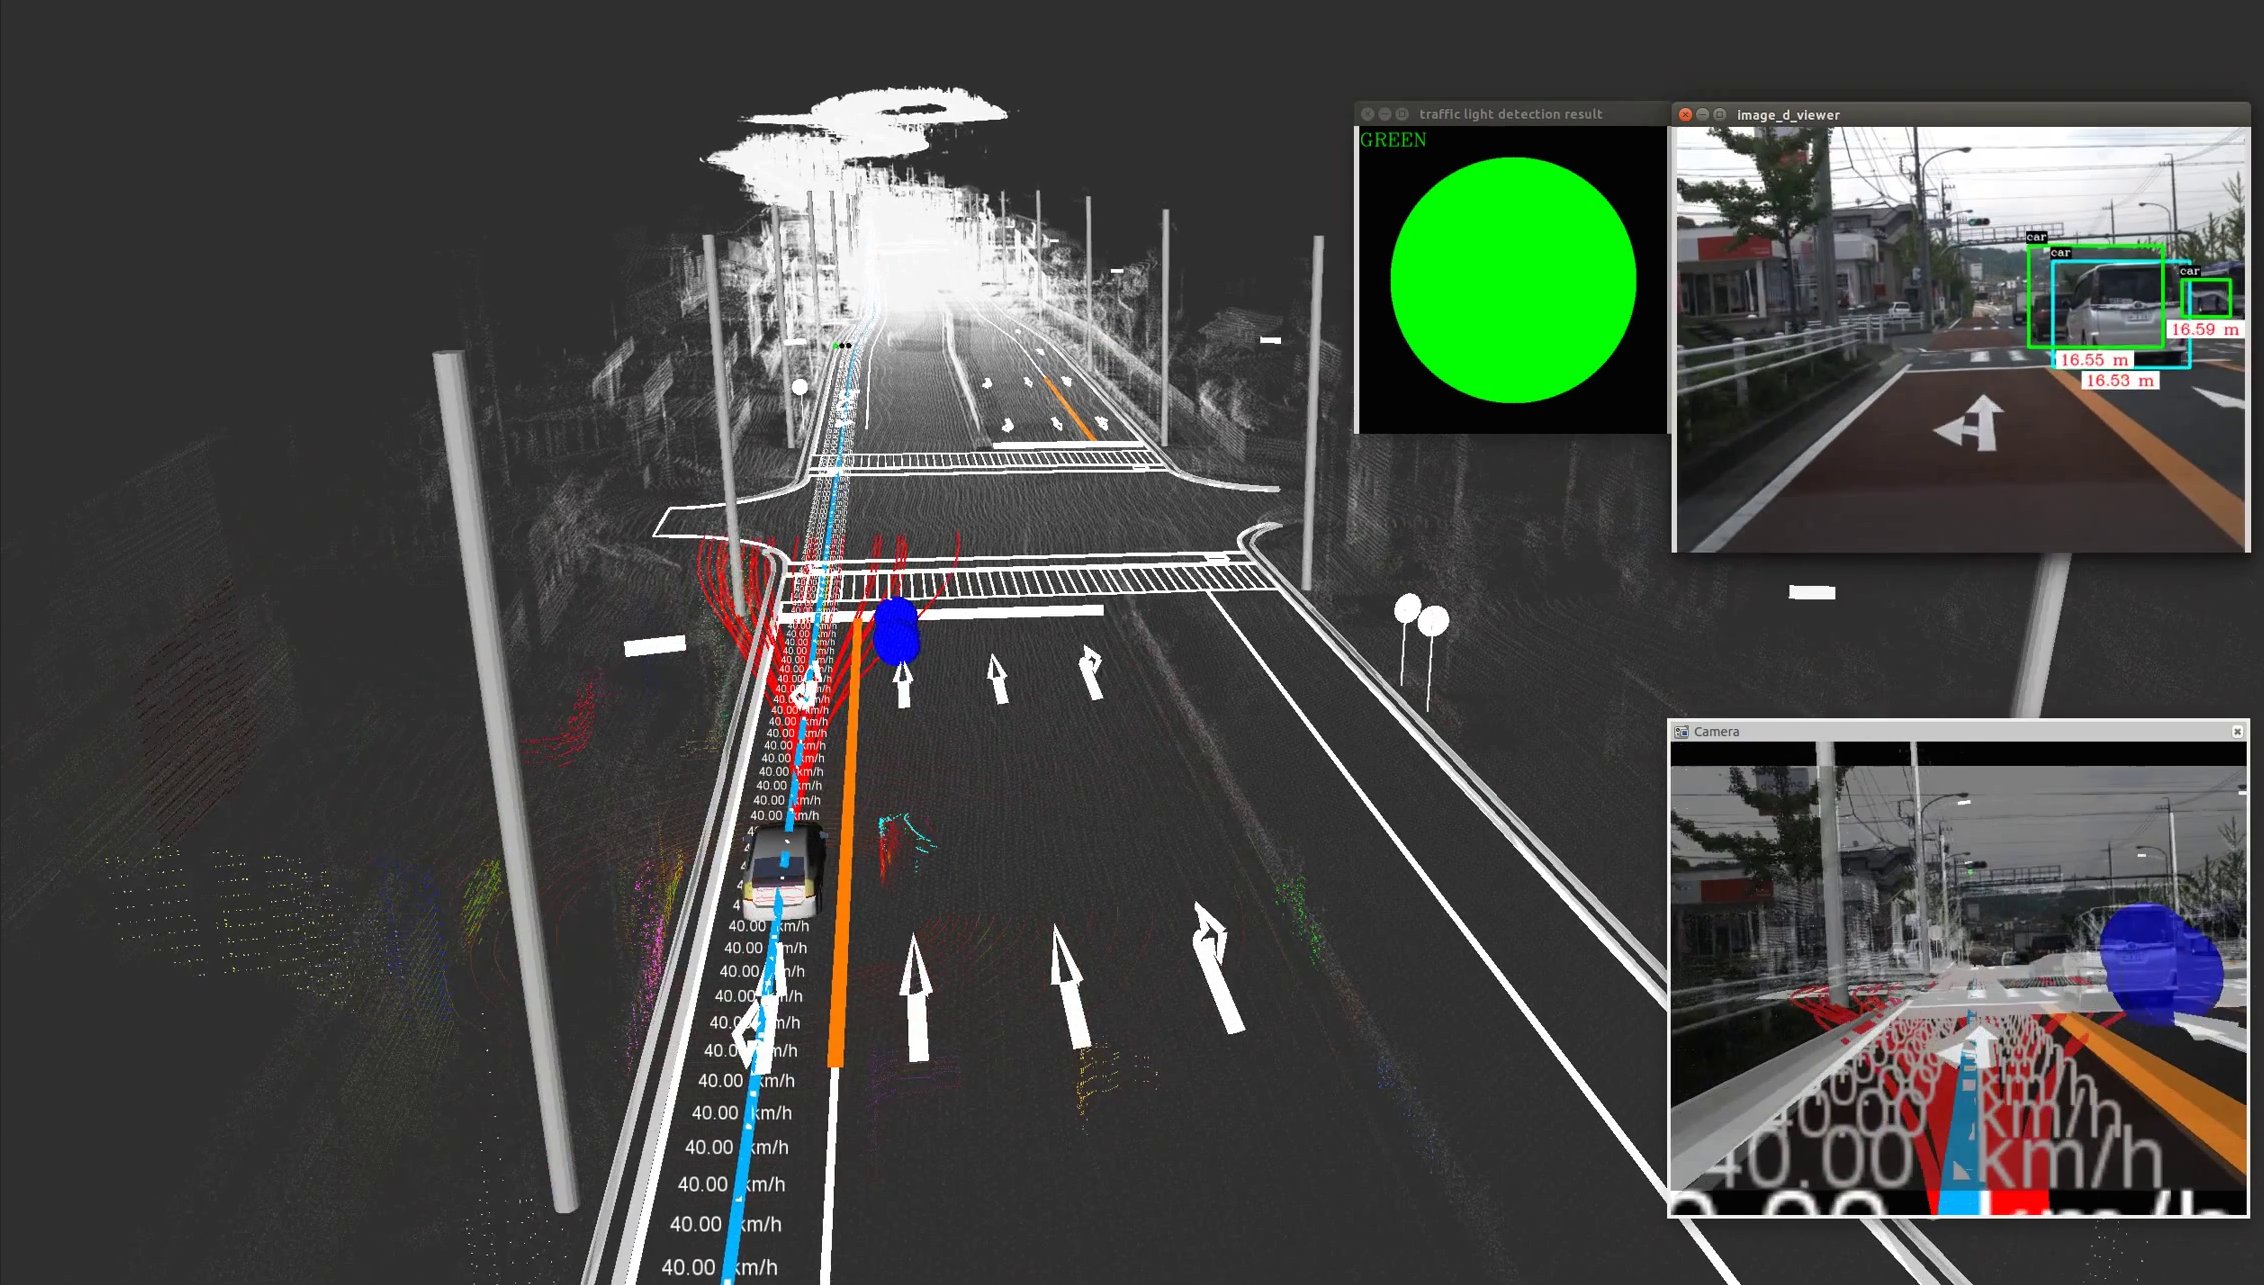
\includegraphics[width = \textwidth]{figures/apex_planning.png}
 	\vspace{-10pt}
 	\caption{ROS APEX planning implementation GUI.}
 	\vspace{-10pt}
 	\label{fig:ros}
 \end{figure}
 
 One real-world example of an AV software bug related to plan execution was highlighted by the first ever crash between AVs at the Urban Challenge \cite{fletcher2008cornell}. At the time of the accident, participants noted that there are no known \quotes{formal methods that would allow definitive statements about the completeness or correctness of a vehicle interacting with a static environment, much less a dynamic one} \cite{urmson2008autonomous}. It is beyond the scope of this paper to review the numerous developments in verification and synthesis technology;
 we note attempts exist to reason about the safety of autonomous vehicles in static environments via synthesis \cite{Wongpiromsarn2010}, but such methods cannot currently scale to realistic systems and are extremely conservative. In response the authors of \cite{Wongpiromsarn2010} propose a receding horizon framework, but still rely on coarse grid-based abstractions. Others have sought to verify Adaptive Cruise Control Algorithms (ACC) which severely restrict scenarios in which the car may operate (no lane changes) \cite{nilssoncorrect}. Finally, some research which eschews discretization in favor of continuous linearized dynamics focuses on moving the verification task online \cite{althoff2012}.
 
 
\pagebreak
\part{Vehicle Modeling}
\section{Autonomous Vehicle Software Architecture}
In order to motivate the need for the APEX approach, we first outline the architecture of a typical ADAS/AV control system. 
It is \emph{not} necessary that a vehicle use this \emph{particular architecture} in order to be verified under APEX, but it motivates the key issues involved in obtaining a proof of safety. In the three-layer architecture paradigm \cite{Gat98} which we demonstrate, the planning and control of the vehicle is hierarchical in nature. Each successive layer performs a task over a shorter time horizon. Fig. \ref{fig:tla_new} details this approach to AV architecture.

\begin{figure}[h]
	\centering
	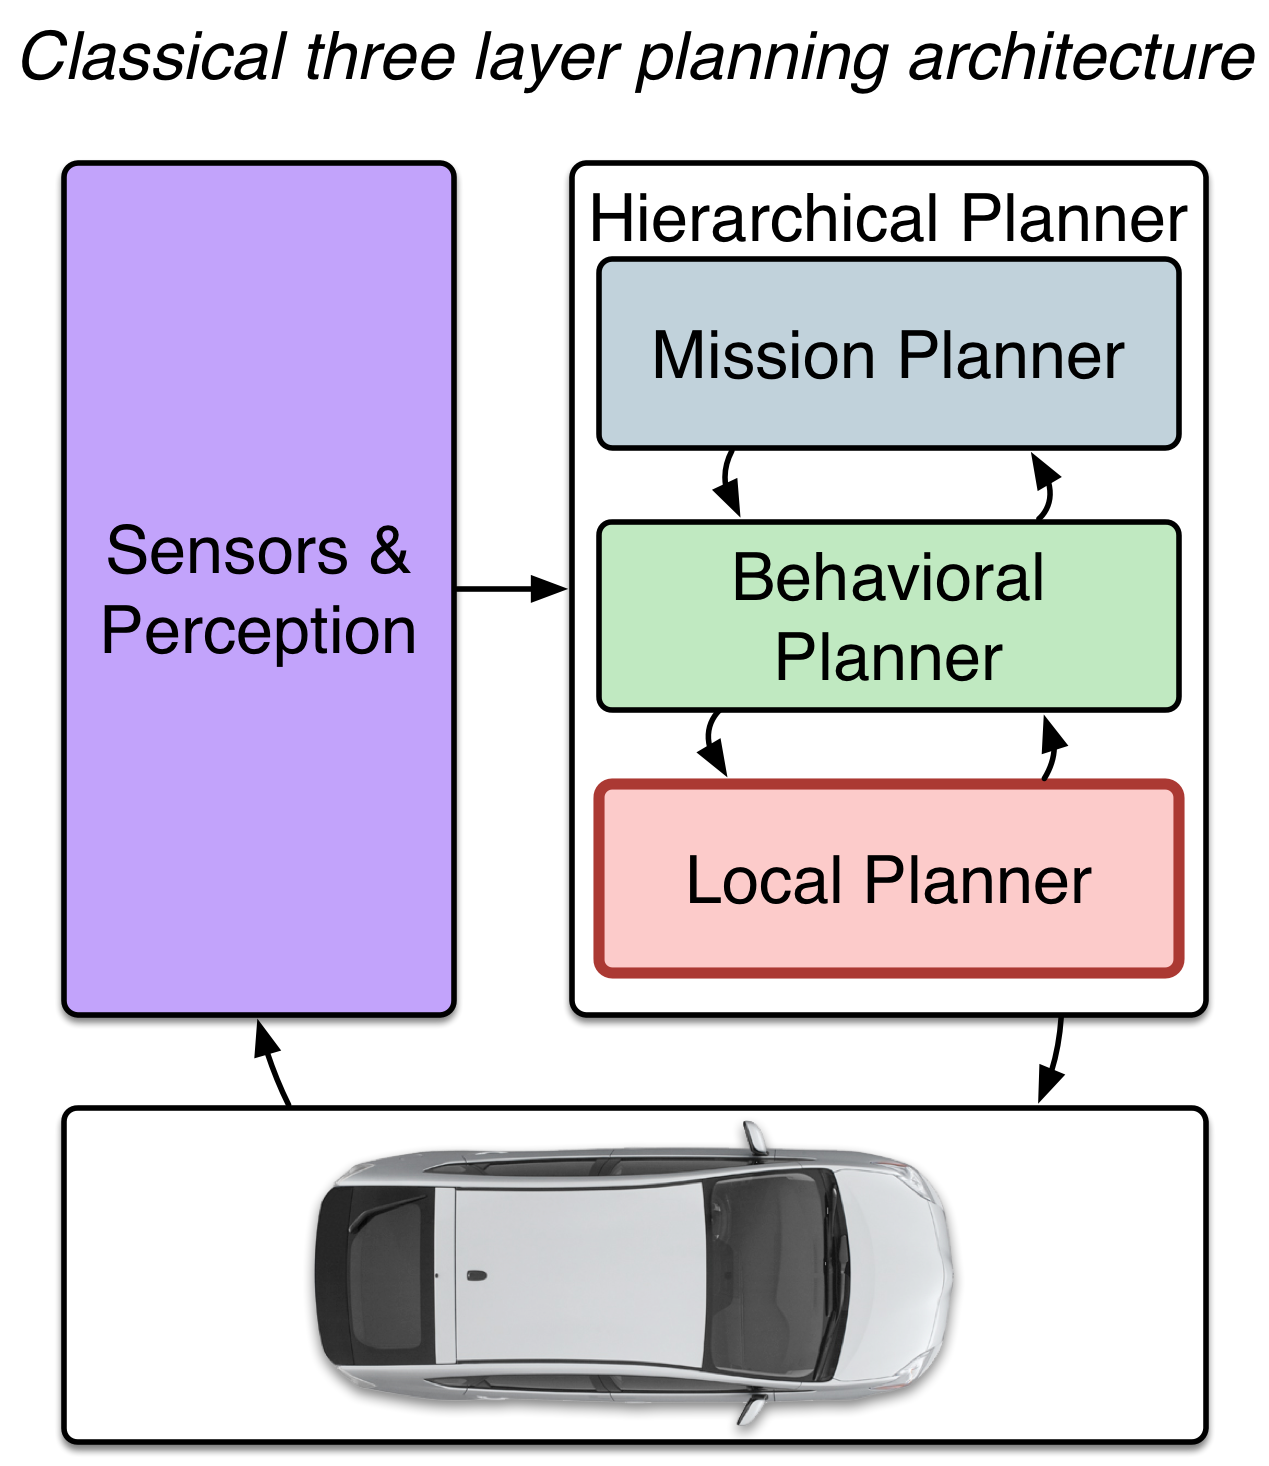
\includegraphics[scale=.3]{figures/tla_new.png}
	\caption{The three layer architecture presented by Gat is widely accepted as a standard means of implementing planning and control for an autonomous vehicle.}
	\label{fig:tla_new}
\end{figure}

At the top level a mission planner is given a mobility goal. Such a goal is typically expressed as a (location, destination) pair. Given this pair the mission planner finds an optimal (or feasible) route through the road network. 

In the next layer, the behavioral planner makes local decisions about how to navigate the road network. For example, if the mission planner informs the behavioral planner that at the next intersection it will need to turn left, the behavioral planner will use a set of rules to determine that the ego vehicle must be in the left lane.
It then provides a sequence of waypoints, or intermediary destinations, to the lower-level local planner. 

Finally, the local planner, or \emph{trajectory planner}, produces a trajectory that connects the vehicle's current pose to the target pose at the next waypoint. 
Here `pose' refers to the combined position, heading and velocity of the vehicle.
Specifically, given a goal pose relative to the vehicle's current pose, the local planner computes a set of candidate smooth trajectories that can lead to the goal pose or near it, then selects a single trajectory and sends it to the vehicle. 
The vehicle itself includes a PID controller (or some other controller) that makes it track the selected trajectory.
\section{Building an Autonomous Vehicle Agent}
To run APEX, we need to capture the AV dynamics, the low level tracking controller, and the planning stack which generates the trajectories for the vehicle to follow. 
\subsection{Modeling}
\label{sec:model}
%We illustrate the usage of APEX by using it to verify several scenarios which cause the ego-vehicle to attempt a lane change maneuver. 
The first step towards verification is a model of the AV.
APEX uses the formalism of nonlinear hybrid systems to describe the AV and other vehicles.
The trajectory tracking controller and AV can be described using ordinary differential equations. 
The discrete nature of the behavioral control layer dictates that we much capture a system with mixed continuous-discrete dynamics. 
We provide a list of symbols used in Table \ref{table:vehiclemodel}.

\begin{table}
	\centering
	\caption{Symbols for Vehicle Model}
	\begin{tabular}{|c|c|c|}
		\hline
		\multicolumn{3}{|c|}{Symbol List} \\ \hline
		 Symbol & Units & Description \\ \hline
		$x_v$ & - & Verification State Vector \\ \hline 
		$x_{sl}$ & - & Lattice Planning State Vector \\ \hline
		$x_p$ & - & Vehicle Pose \\ \hline
		$x_g$ & - & Goal Pose \\ \hline
		$x_f$ & - & Predicted Vehicle Pose \\ \hline
		$p$ & - & Cubic Spline Parameter Vector \\ \hline
		$t_f$ & s & Prediction Horizon \\ \hline
		$m$ & kg & Vehicle Mass \\ \hline
		$l_r$ & m & Rear Wheelbase \\ \hline
		$l_f$ & m & Front Wheelbase \\ \hline
		$I_z$ & kg m$^2$ & Moment of Inertia \\ \hline
		$C_f$ & N/rad & Front Cornering Stiffness  \\ \hline
		$C_r$ & N/rad & Rear Cornering Stiffness \\ \hline
		$\beta$ & rad & Slip Angle \\ \hline
		$\Psi$ & rad & Heading Angle \\ \hline
		$v$ & m/s & Velocity \\ \hline
		$s_x$ & m & Position, x \\ \hline
		$s_y$ & m & Position, y \\ \hline
		$\delta$ & rad & Steering Angle \\ \hline
		$\epsilon_x$ & m & Tracking Error, x \\ \hline
		$\epsilon_y$ & m & Tracking Error, y \\ \hline
		$v_w$ & rad/s & Steering Angle Velocity \\ \hline 
		$a_x$ & m/s$^2$ & Longitudinal Acceleration \\ \hline
		$\kappa$ & rad/m & Curvature \\ \hline
		$s_f$ & m & Arc Length \\ \hline	
	\end{tabular}	
	\label{table:vehiclemodel}
\end{table}

\subsubsection{Ego Vehicle Model}
%To demonstrate the ability of APEX to investigate more complex vehicle models 
APEX uses a non-linear 7 degree of freedom bicycle model \cite{Rajamani2011} in order to describe the ego-vehicle. 
Higher order models can be supported in the future, and of course the parameters of the base model can be customized in order to match specific vehicles. 
See Fig. \ref{fig:bike}. 
The input to such a model is steering angle velocity and linear velocity, the output is vehicle state as a function of time. 

\begin{figure}[b]
	\centering
	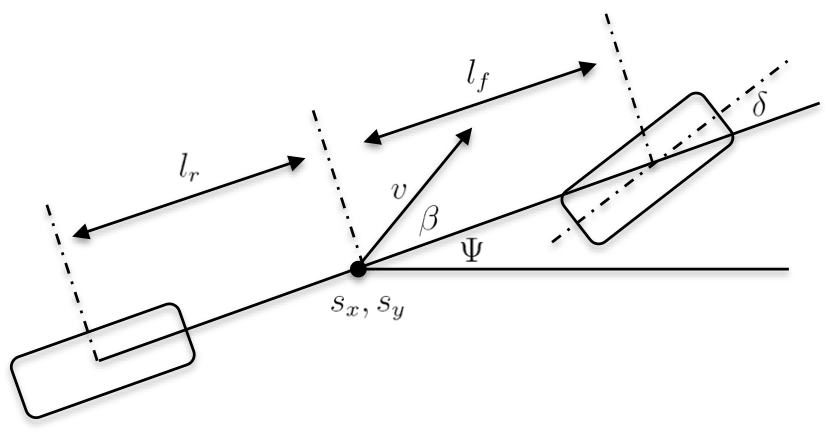
\includegraphics[scale=.6]{figures/bicycle_model.png}
	\caption{Nonlinear bicycle model describing the statespace for the APEX approach to vehicle dynamics}
	\label{fig:bike}
\end{figure}

The state vector describing the vehicle is described in equations (1)-(7). 
The variable \(\beta\) is the slip angle at the center of mass, \(\psi\) is the heading angle, \(\dot{\psi}\) is the yaw rate, \(v\) is the velocity, \(s_x\) and \(s_y\) are the x and y positions, and \(\delta\) is the angle of the front wheel. In the formulation of [6], the inputs to the system are \(a_x\), the longitudinal acceleration, and \(v_w\) the rotational speed of the steering angle. 
%The \(y\) terms represent disturbances to the system. For example \(y_{\beta}\) and \(y_{\dot{\psi}}\) represent disturbances to the slip angle at the center of mass and the yaw rate. 
\begin{equation}
	x_v = (\beta,\Psi,\dot{\Psi}, v, s_x, s_y, \delta)
\end{equation}	

 The state equations for the system as described in \cite{Althoff2014} are:
\begin{equation}
	\label{eqn:beta}
	\dot{\beta}=\left(\frac{C_rl_r-C_fl_f}{mv^2} \right)\dot{\psi}+\left(\frac{C_f}{mv} \right)\delta-\left(\frac{C_f+C_r}{mv} \right)\beta
\end{equation}
\begin{gather}
	\label{eqn:psi}
	\ddot{\psi}=\left(\frac{C_rl_r-C_fl_f}{I_z} \right)\beta-\left(\frac{C_fl_f^2-C_rl_r^2}{I_z} \right)\left(\frac{\dot{\psi}}{v} \right) \notag \\
	+\left(\frac{C_fl_f}{I_z} \right)\delta
\end{gather}
\begin{equation}
	\label{eqn:v}
	\dot{v}=a_x
\end{equation}
\begin{equation}
	\label{eqn:sx}
	\dot{s_x}=v\cos{(\beta+\psi)}
\end{equation}
\begin{equation}
	\label{eqn:sy}
	\dot{s_y}=v\sin{(\beta+\psi)}	
\end{equation}	
\begin{equation}
	\label{eqn:delta}
	\dot{\delta}=v_w
\end{equation}

%We note that in order to analyze the system we represent \(\ddot{\psi}\) as two first order differential equations. Thus we write:
%\begin{gather}
%	\dot{\psi}_{dot}=\left(\frac{C_rl_r-C_fl_f}{I_z} \right)\beta-\left(\frac{C_fl_f^2-C_rl_r^2}{I_z} \right)\left(\frac{\dot{\psi}}{v} \right) \notag \\+\left(\frac{C_fl_f}{I_z} \right)\delta\\
%	\dot{\psi}=\psi_{dot}
%\end{gather}
%Finally, one must substitute \(\psi_{dot}\) for each appearance of \(\dot{\psi}\) in the other state equations.

\subsubsection{Vehicle Parameters}
The parameters \(C_f,C_r\) and \(l_f, l_r\) describe respectively the cornering stiffness and distances from the center of gravity to the axles respectively; the subscripts $f,r$ denote whether the parameter is defined for the front or rear of the vehicle. The moment of inertia, \(I_z\) and the vehicle mass, \(m\) are experimentally determined constants \cite{Snider2009}. 
 The kinematic bicycle model considers the two front wheels and two rear wheels of the vehicle to move in unison, with steering provided by the front wheels only. Furthermore, Each abstracted wheel is located along the center of the vehicle's body. Table \ref{table:vehiclep} contains the validated vehicle parameters as given in \cite{Althoff2014}. It is possible to obtain such parameters and replace these constants in order to investigate specific vehicle characteristics. 

\begin{table}[h]
	\centering
	\caption{Parameters of Example Ego Vehicle \cite{Althoff2014}}
	\label{table:vehiclep}
	\begin{tabular}{|c|c|c|c|c|c|}
		\hline
		\multicolumn{6}{|c|}{Vehicle Parameters} \\ \hline
		\textit{$m$(kg)} & \textit{$I_z$(kg*m$^2$)} & \textit{$C_f$(N/rad)} & \textit{$C_r$(N/rad)} & \textit{$l_f$(m)} & \textit{$l_r$(m)} \\ \hline
		2273 & 4423 & 10.8e4 & 10.8e4 & 1.292 & 1.515 \\ \hline
	\end{tabular}	
\end{table}

\subsubsection{Tracking Controller}
A simple trajectory tracking controller is included with the APEX vehicle model. Trajecotry tracking controllers guide a vehicle along a geometrically defined cubic spline by apply steering and longitudinal acceleration inputs. A successful path tracking algorithm maintains vehicle stability and attempts to minimize the error between the desired trajectory and actual trajectory. The parameters computed for this controller when implemented and validated on a typical crossover SUV \cite{Althoff2014} are presented in Table \ref{table:controller}. 

\begin{table}[h]
	\centering
	\caption{Controller Parameters \cite{Althoff2014}}
	\label{table:controller}
	\begin{tabular}{|c|c|c|c|c|c|}
		\hline
		\multicolumn{6}{|c|}{Controller Parameters} \\ \hline
		$k_1$ & $k_2$ & $k_3$ & $k_4$ & $k_5$ & $k_6$ \\ \hline
		2 & 12 & 4 & 2 & 1 & 1.515 \\ \hline
	\end{tabular}	
\end{table}

%Thus, the feedback to the system are the lateral and longitudinal tracking errors. We derive the following results as in  \cite{Snider2009}:
%\begin{gather}
%	\epsilon_x=cos{(\Psi_d)}(s_{x,d}-s_x) +sin{(\Psi_d)}(s_{y,d}-s_y)
%	\\
%	\epsilon_y=-sin{(\Psi_d)}(s_{x,q}-s_x)+cos{(\Psi_d)}(s_{y,d}-s_y)
%\end{gather}



%Through the lateral tracking error, and desired trajectory we can then compute the desired rate of change of the angle of the front wheel with respect to time. This enables the computation of rate of change of the rotational speed of the steering %angle. We note that the relevant parameters are again defined using the validated model and are compiled in Table \ref{table:controller}.
%\begin{gather}
%	\delta_d=k_1 \epsilon_y+k_2(\Psi_d-\Psi)+ k_3(\dot{\Psi_d}-\dot{\Psi})
%	\\
%	v_w=k_4(\delta_d-\delta)
%	\end{gather}

%The longitudinal acceleration is simply defined by the tracking error between the actual velocity and the desired velocity.
%\begin{gather}
%	a_x=k_5\epsilon_x+k_6(v_d-v)
%\end{gather}

Using the approach in \cite{Snider2009} and \cite{Althoff2014} the control inputs for longitudinal acceleration (pressing the accelerator) and steering angle velocity (turning the steering wheel) can be computed as $v_w$ and $a_x$ respectively. 
\begin{gather}
	v_w=k_1(cos{(\Psi_d)}(s_{y,d}-s_y-w_y)-sin{(\Psi_d)}(s_{x,d}-s_x-w_x)) \notag \\ +k_2(\Psi_d-\Psi-w_{\Psi}) \notag \\ +k_3(\dot{\Psi_d}-\dot{\Psi}-w_{\psi})-k_4(\delta-w_{\delta})
	\\
	a_x=k_5(cos{(\Psi_d)}(s_{x,d}-s_x-w_x)+sin{(\Psi_d)}(s_{y,d}-s_y-w_y)) \notag \\ +k_6(v_d-v-w_v)
\end{gather}

We note that we cannot use traditional linear systems techniques or sum of squares optimizations to directly find a Lyapunov function for this system because of the obvious non-linearity and non-polynomial form of the governing ordinary differential equations. Instead we will seek to show stability and safety properties using reachability and model checking analysis.

\subsubsection{Planning}
In APEX we provide a validated planning stack which can be run on a real vehicle. The planning strategy is hierarchical and includes: mission planning, behavioral planning, and local planning. In this section we will focus on the local planner because it is the layer which connects directly to the tracking controller for the vehicle. The local planner is used to generate smooth trajectories which a non-holonomic dynamically constrained vehicle is capable of following. Our planning stack utilizes the methods outlined in 
\cite{McNaughton_2011_6927} commonly known as state-lattice planning with cubic spline trajectory generation.
%\cite{nagy2001trajectory}, , \cite{ferguson2008motion} 
\begin{figure}[t]
	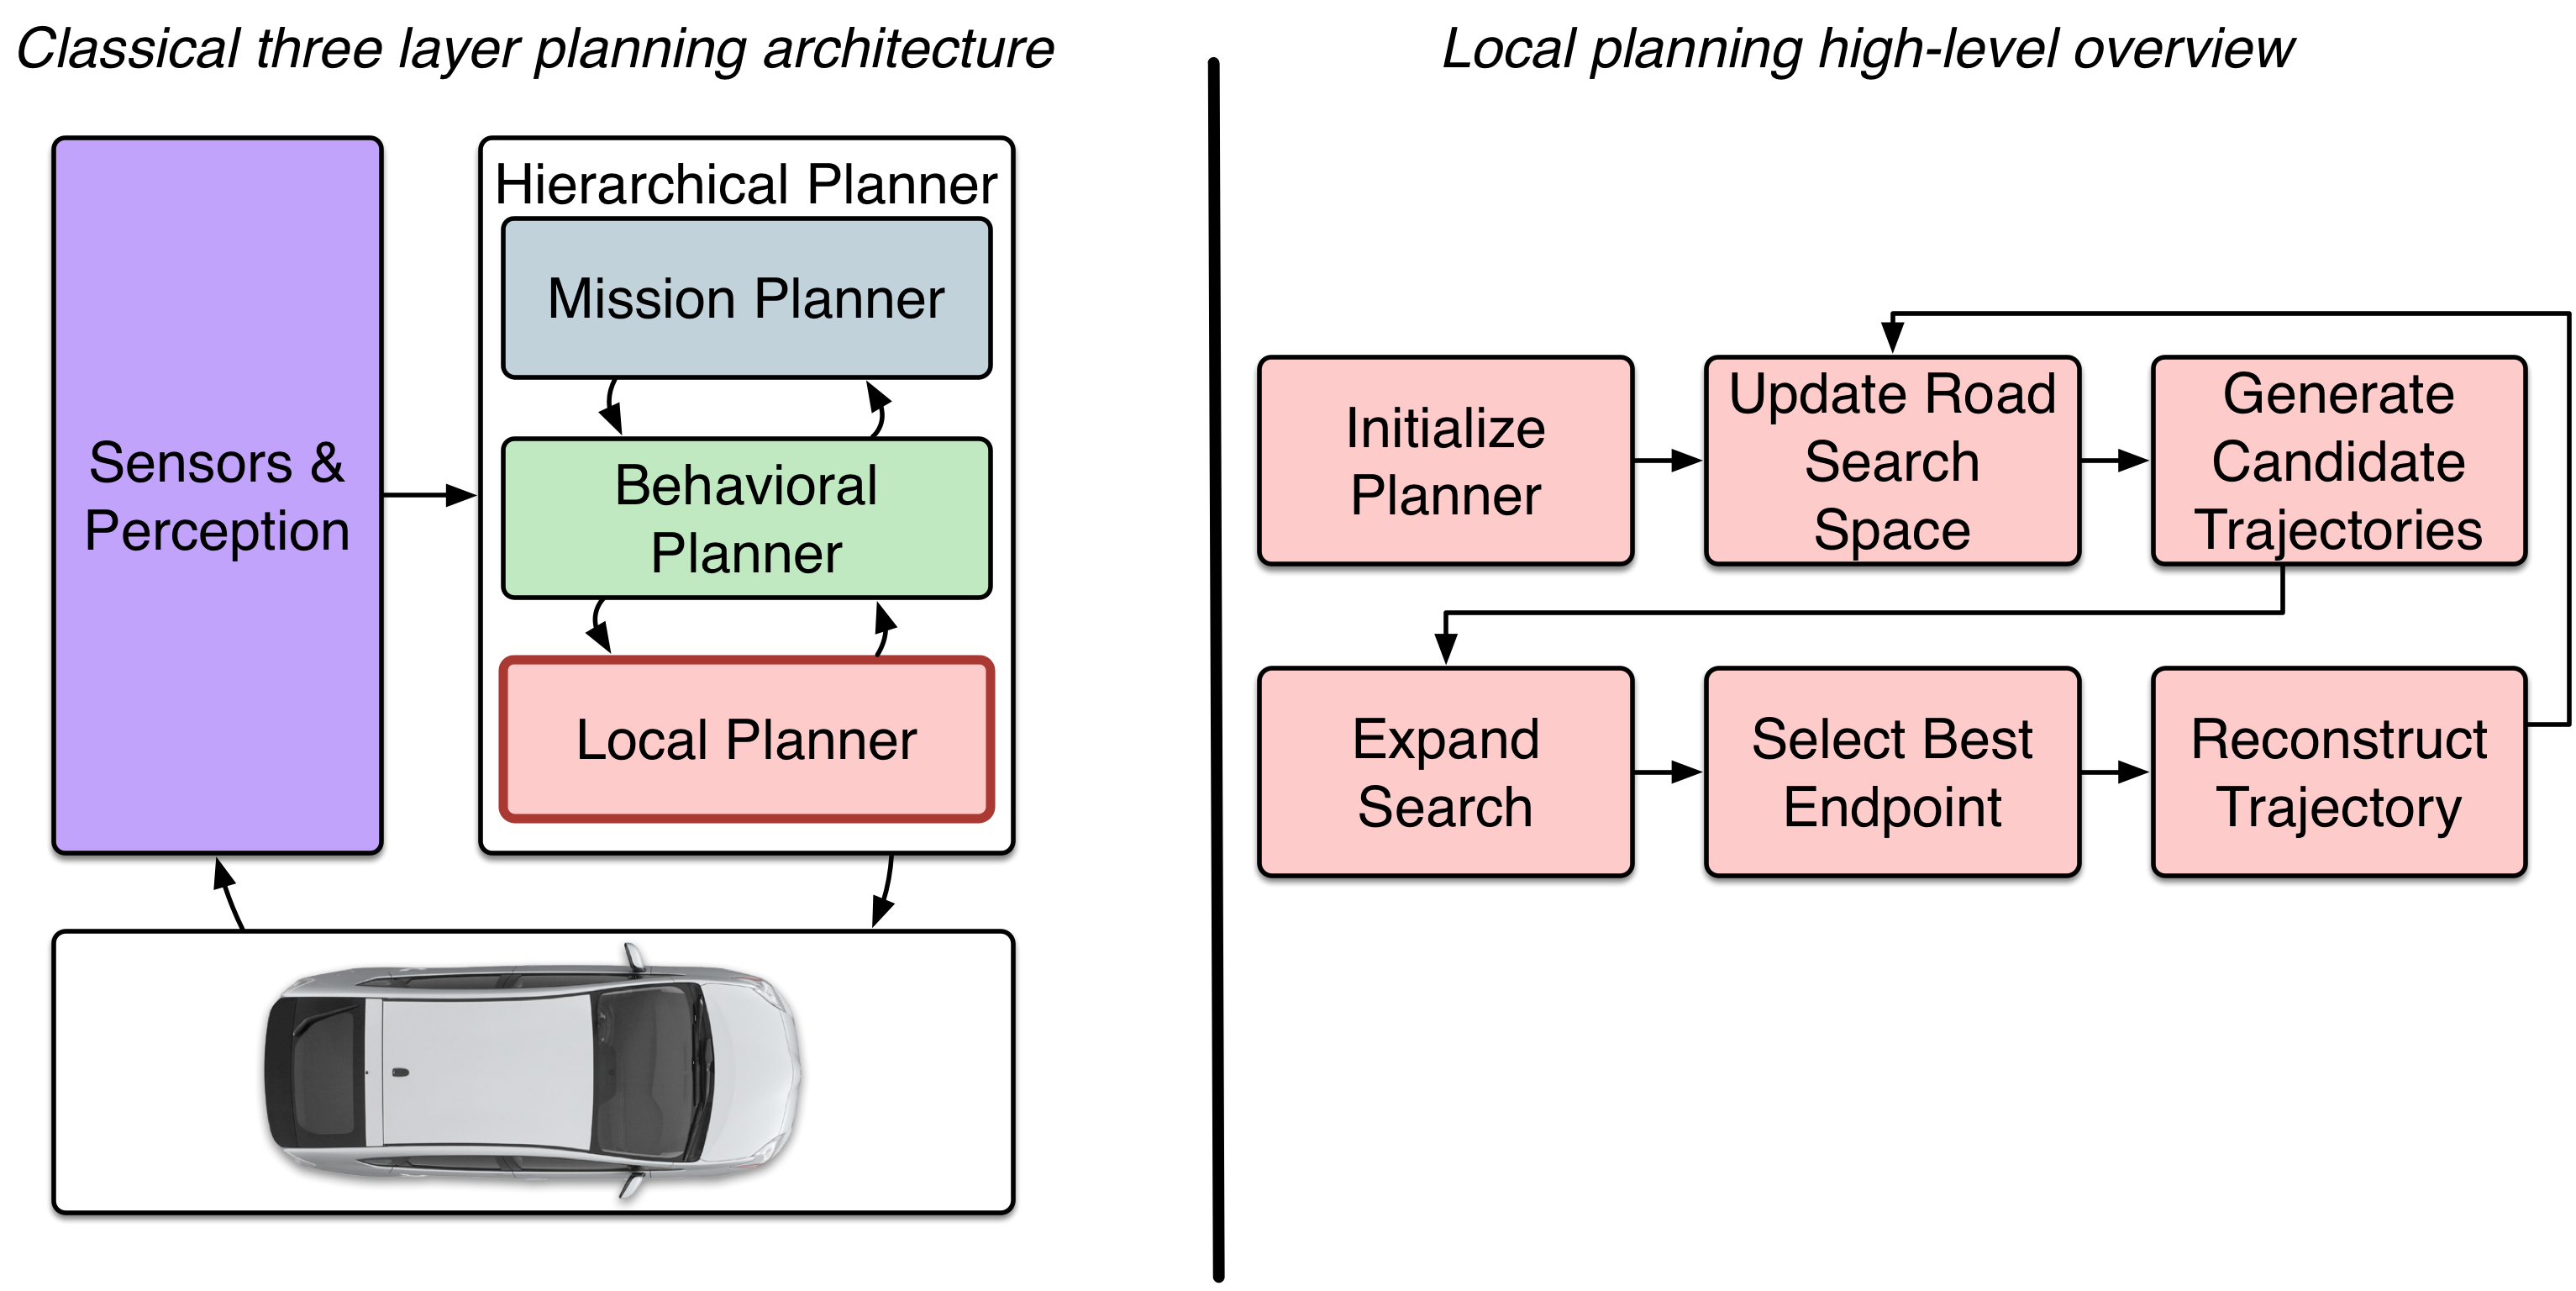
\includegraphics[width=\columnwidth]{figures/planning.png}
	\caption{Details of a local planning algorithm and used by AVs employing state lattice planning}
	\vspace{-10pt}
	\label{fig:planning}
\end{figure}

Each execution of the planner requires as an input the current state of the vehicle and a goal state as defined by the behavioral planner. We note that we will call the vehicle state $x_{sl}$ because it does not necessarily have to be the same as the model used for verification (although it can be); because the planner must run online, in real-time, lower order models are often substituted here. In this implementation we define $x_{sl}$ as:
\begin{equation}
	x_{sl}=(s_x, s_y, v, \Psi, \kappa)
\end{equation}

Where $s_x$ and $s_y$ are the x and y positions of the center of mass, $v$ is the velocity, $\Psi$ is the heading angle, and $\kappa$ is the curvature. We note that the state equations involve an additional constant, $L$ which is the wheelbase of the vehicle.
Where the state equations are described as:
\begin{equation}
	\dot{x}= v*cos(\Psi)
\end{equation}
\begin{equation}
	\dot{y} = v*sin(\Psi)
\end{equation}
\begin{equation}
	\dot{\theta}= \kappa*v
\end{equation}
\begin{equation}
	\dot{\kappa} = \frac{\dot{\Psi}}{L}
\end{equation}

The local planner's objective is then to find a feasible trajectory from the initial state defined by the tuple $x_{sl}$ to a goal pose $x_{p}$ defined as:
\begin{equation}
	x_{p} = (s_x,s_y,\Psi)
\end{equation}

In this formulation we limit trajectories to a specific class of parameterized curves known as cubic splines. A cubic spline is defined as a function of arc length:
\begin{equation}
	\kappa(s) = \kappa_0 + a \kappa_1 s + b \kappa_2 s^2 + c \kappa_3 s^3
\end{equation}

Note that there are four free parameters $(a,b,c,s_f)$ and our goal posture has four state variables. Thus, a cubic spline is a minimal polynomial that can be assured to produce a trajectory from the current position to the goal position (if it is kinematically feasible). For any particular state, goal pair there are two steps necessary to compute the parameters. First, it is necessary to produce an initial guess. There are several approaches available such as using a neural network, lookup table, or a simple heuristic. In this case we adapt a heuristic from Nagy and Kelly \cite{nagy2001trajectory} such that it is compatible with a stable parameter formulation presented by McNaughton \cite{McNaughton_2011_6927}. The stable reparameterization is defined as:
\begin{gather}
	\kappa(0)=p_0\\
	\kappa(s_f/3)=p_1\\
	\kappa(2s_f/3)=p_2\\
	\kappa(s_f)=p_3
\end{gather}

Where the parameters $(a,b,c,s_f)$ can now be expressed as:
\begin{gather}
	a(p)=p_0\\
	b(p)=-\frac{11p_0 - 18p_1+9p_2-2p_3}{2s_f}\\
	c(p)=\frac{9*(2p_0-5p_1+4p_2-p_3)}{2s_f^2}\\
	d(p)=-\frac{9(p_0-3p_1 +3p_2-p_3)}{2s_f^3}
\end{gather}
Which results in the following initialization heuristic:
\begin{gather}
	p_0=\kappa_0=\kappa_i\\ 
	p_1=\kappa_1= \frac{1}{49}(8b(s_f-s_i)-26\kappa_0-\kappa_3)\\
	p_2=\kappa_2=\frac{1}{4}(\kappa_3-2\kappa_0+5\kappa_1)\\
	p_3=\kappa_3=\kappa_f
\end{gather}

Finally, with an initial guess in hand, and a stable re-parameterization the local planner can solve a simple gradient descent problem to drive the vehicle to the goal posture. 
%We will be concerned with computing trajectories which lead from an initial state $x_i$ to a final state $x_t$ within a finite time horizon. The final state state boundary constraints which are given by the mission planner are defined by the following vector:
%\begin{equation}
%x_c=[s_x,s_y, \Psi]
%\end{equation}
%A prediction of the vehicles final state (using Euler's method) due to the control input is:
%\begin{equation}
%x_f(p,x)=x_i+\int_{t_0}^{t_f}\dot{x}(x,p)dt
%\end{equation}
%The goal of the algorithm is to drive the following equation to zero:
%\begin{equation}
%C(x,p)=x_c-x_f(p,x)
%\end{equation}
%
%We then note that $\Delta x = x_f(p,x)-x_i$ is determined by a function $f(x(p,x))$ which can be linearized such that $\Delta x = \frac{df}{dp}\Delta p$. Thus, we can iteratively update the parameters vector $p$ by the following equation:
%\begin{equation}
%	\Delta p = \frac{df}{dp}^{-1} \Delta x
%\end{equation}
%We now have a methodology for computing parameter updates, we note that the function $f(x(x,p)$ cannot be computed directly, but numerically-based algorithms exist which simplify matters. An interested reader may find the details in \cite{Howard_2009_6434}

%In Algorithm \ref{algo:estJacob} we provide the generateCorrection() function with an estimate of the Jacobian. This calculation is done numerically using a forward difference partial derivative estimate. Note that each iteration of the for loop will provide a column of the Jacobian.
%\begin{algorithm}
%	\caption{Estimate Jacobian}
%	\label{algo:estJacob}
%	\begin{algorithmic}
%		\State \textbf{estimateJacobian ($x_t, x_{t+\Delta t}, x_{goal}, u(p,x), \Delta t$)}
%		\State $ m \gets size(p)$
%		\For {$i=0; i< m; i++$}
%		\State $\frac{\delta \Delta x_{t+\Delta t}(p)}{\delta p[i]} \gets \frac{\Delta x_{t+\Delta t}(p[j]+h,p)-\Delta x_{t+\Delta t}(p)}{h}$
%		\EndFor
%		\State \Return {$\frac{\delta \Delta x_{t+\Delta t}(p)}{\delta p}$}
%	\end{algorithmic}
%\end{algorithm}	
%
%\begin{algorithm}
%		\caption{Convergence Criteria for Trajectory Generation}
%		\label{algo:checkConvergence}
%		\begin{algorithmic}
%			\State \textbf{generateCorrection ($x_t, x_{t+\Delta t}, x_{goal}, u(p,x), \Delta t$)}
%			\While {checkConvergence() = FALSE}
%			\State $\Delta x_{t+\Delta t} \gets x_{goal}-\left[x_t+\int_{t}^{t+\Delta t}f(x(t),u(p,x,t),t)dt\right]$
%			\State $\frac{\delta \Delta x_{t+\Delta t}(p)}{\delta p} \gets$ estimateJacobian()
%			\State $\Delta p = \gets -\frac{\delta \Delta x_{t+\Delta t}(p)}{\delta p}^{-1} \Delta x_{t+\Delta t}$
%			\State $ p \gets p + \Delta p$
%			\EndWhile
%			\State \Return {$p$}
%		\end{algorithmic}
%		
%\end{algorithm}
%In Algorithm \ref{algo:checkConvergence} we compute the difference between our forward motion models prediction of the future state of the vehicle and desired goal. While this difference does not satisfy the convergence criteria we update the control input parameters. Informally this is achieved by solving a system of equations which approximates how the state error will change with respect to small changes in the control parameters.

	
Thus, we can now compute a set of parameterized trajectories which may each be evaluated to test for safety and optimality. A description of these aspects of the planner may be found in \cite{McNaughton_2011_6927} and such a cost function can obviously be modified based on the goals of the design team. 
We note that our algorithm implementation is parallelized using OpenMP such that multiple trajectories (with goals regularly sampled around the initial goal) may be evaluated simultaneously. Furthermore, with small changes we can also support quintic splines which expand the variety of possible maneuvers and are more suitable for high speed driving. Figure \ref{fig:traj_gen} shows an example of a trajectory generation instance.
\begin{figure}[t]
	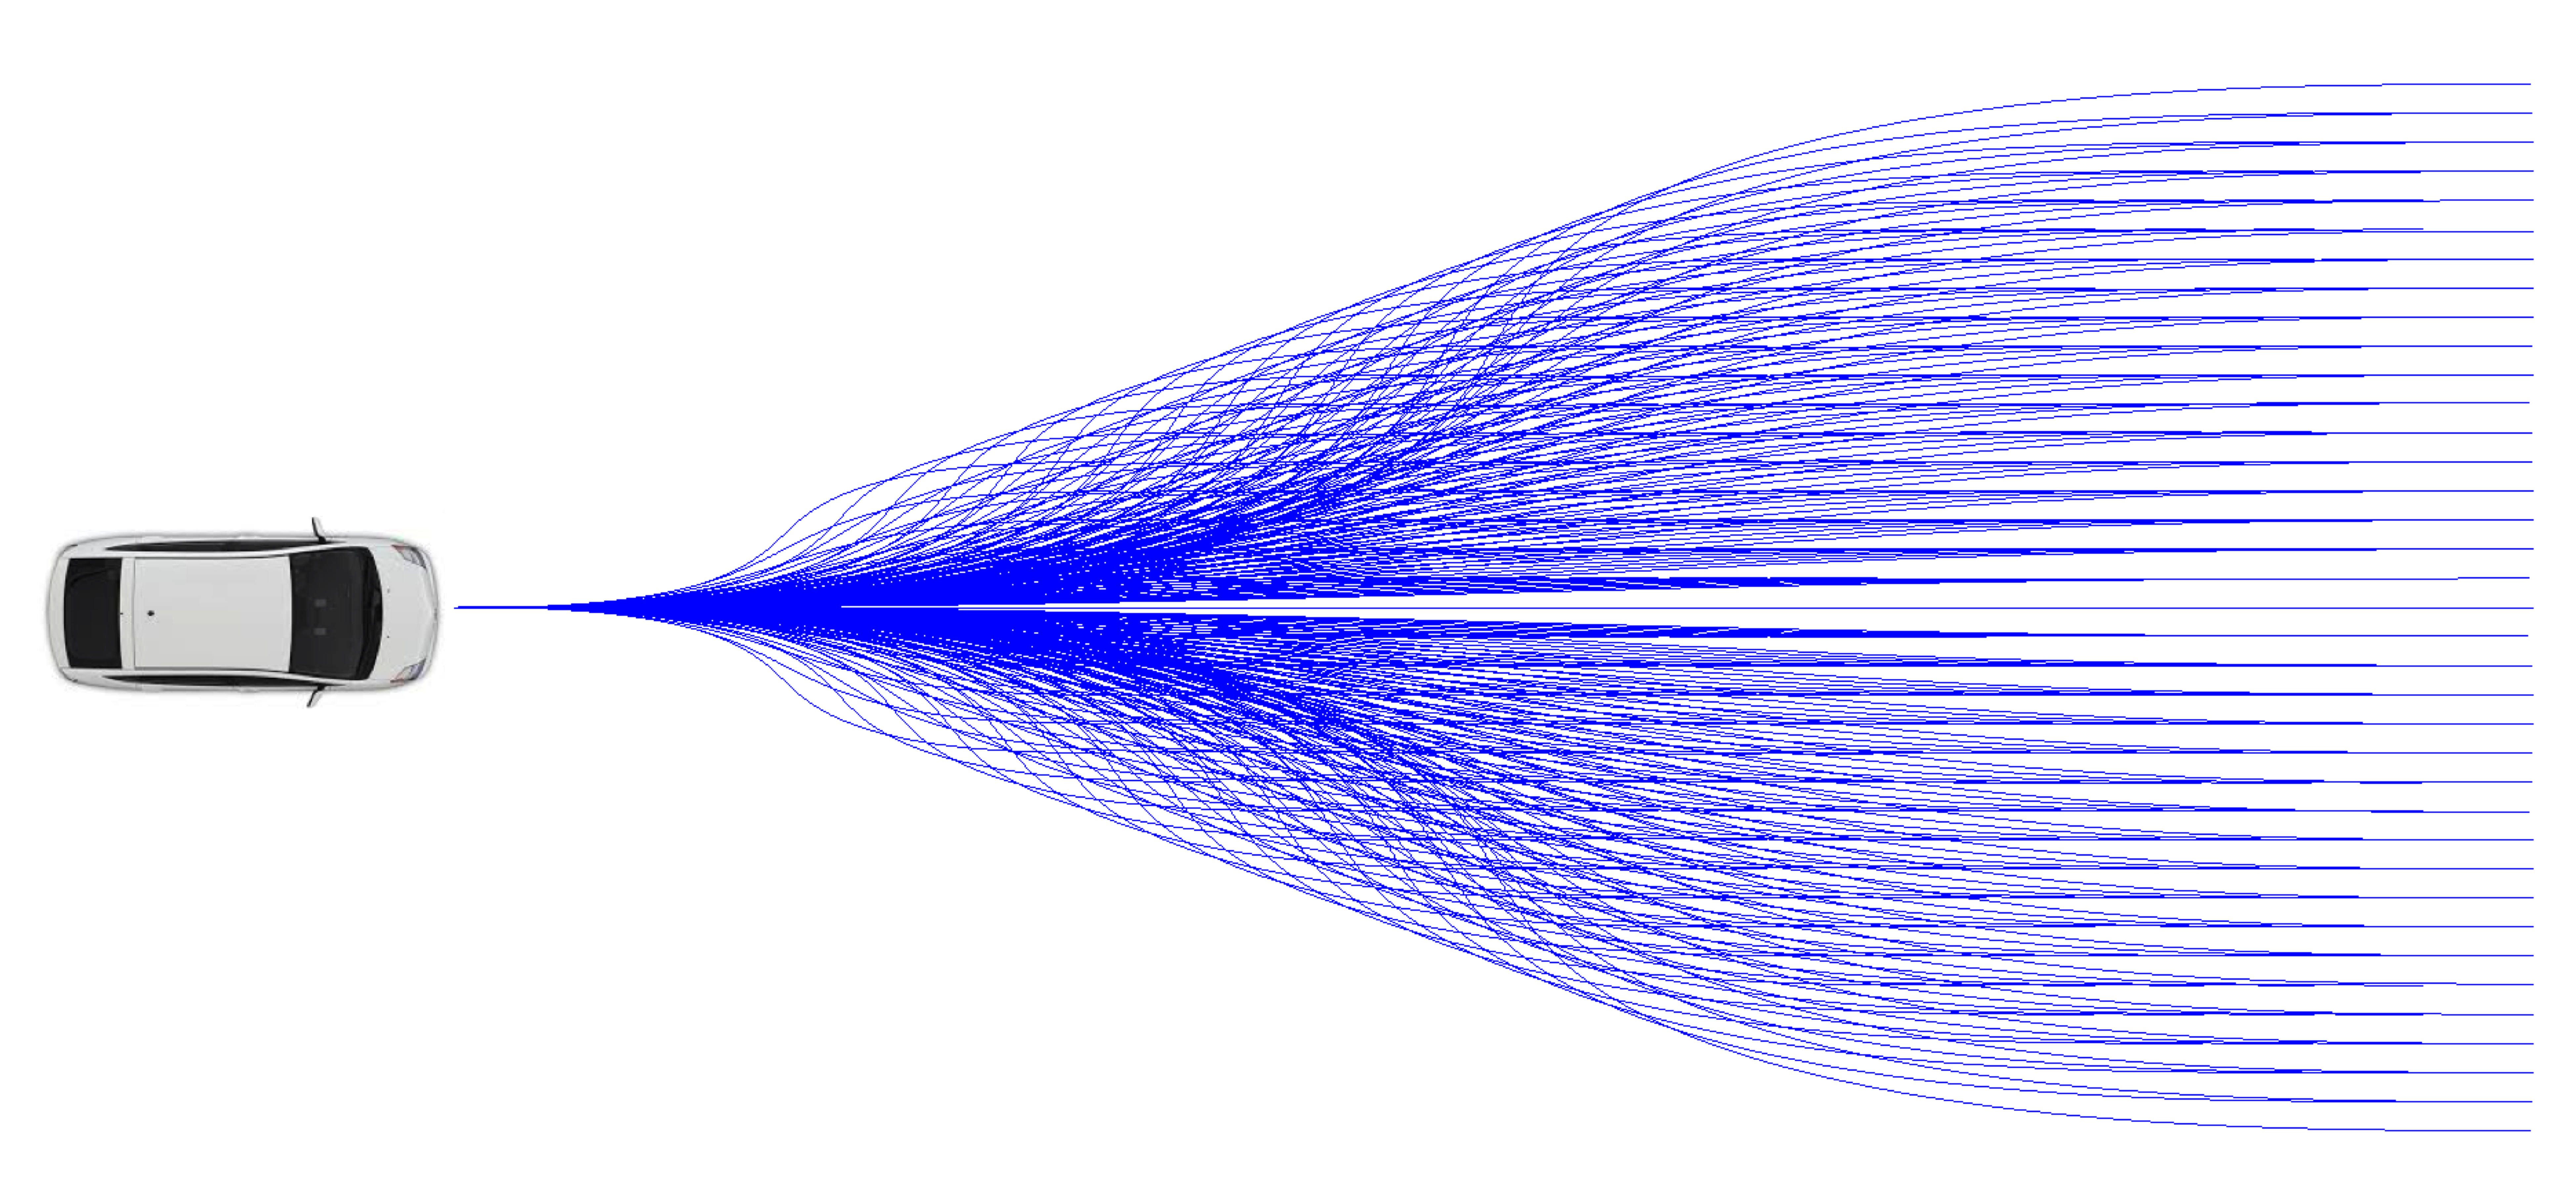
\includegraphics[width=\columnwidth]{figures/traj_gen.png}
	\vspace{-20pt}
	\caption{Output of an execution (10 Hz) of the trajectory generator, a single trajectory will be chosen from this set.}
	\label{fig:traj_gen}
\end{figure}


\pagebreak
\part{Tree Based Verification}
\section{Case Study 1: SAE 2016}

\pagebreak
\part{Composable Hybrid Agents}
\section{Case Study 2}

\pagebreak

\part{Implementation}
\section{APEX Tool}
\subsection{The APEX Approach}
\begin{figure}
	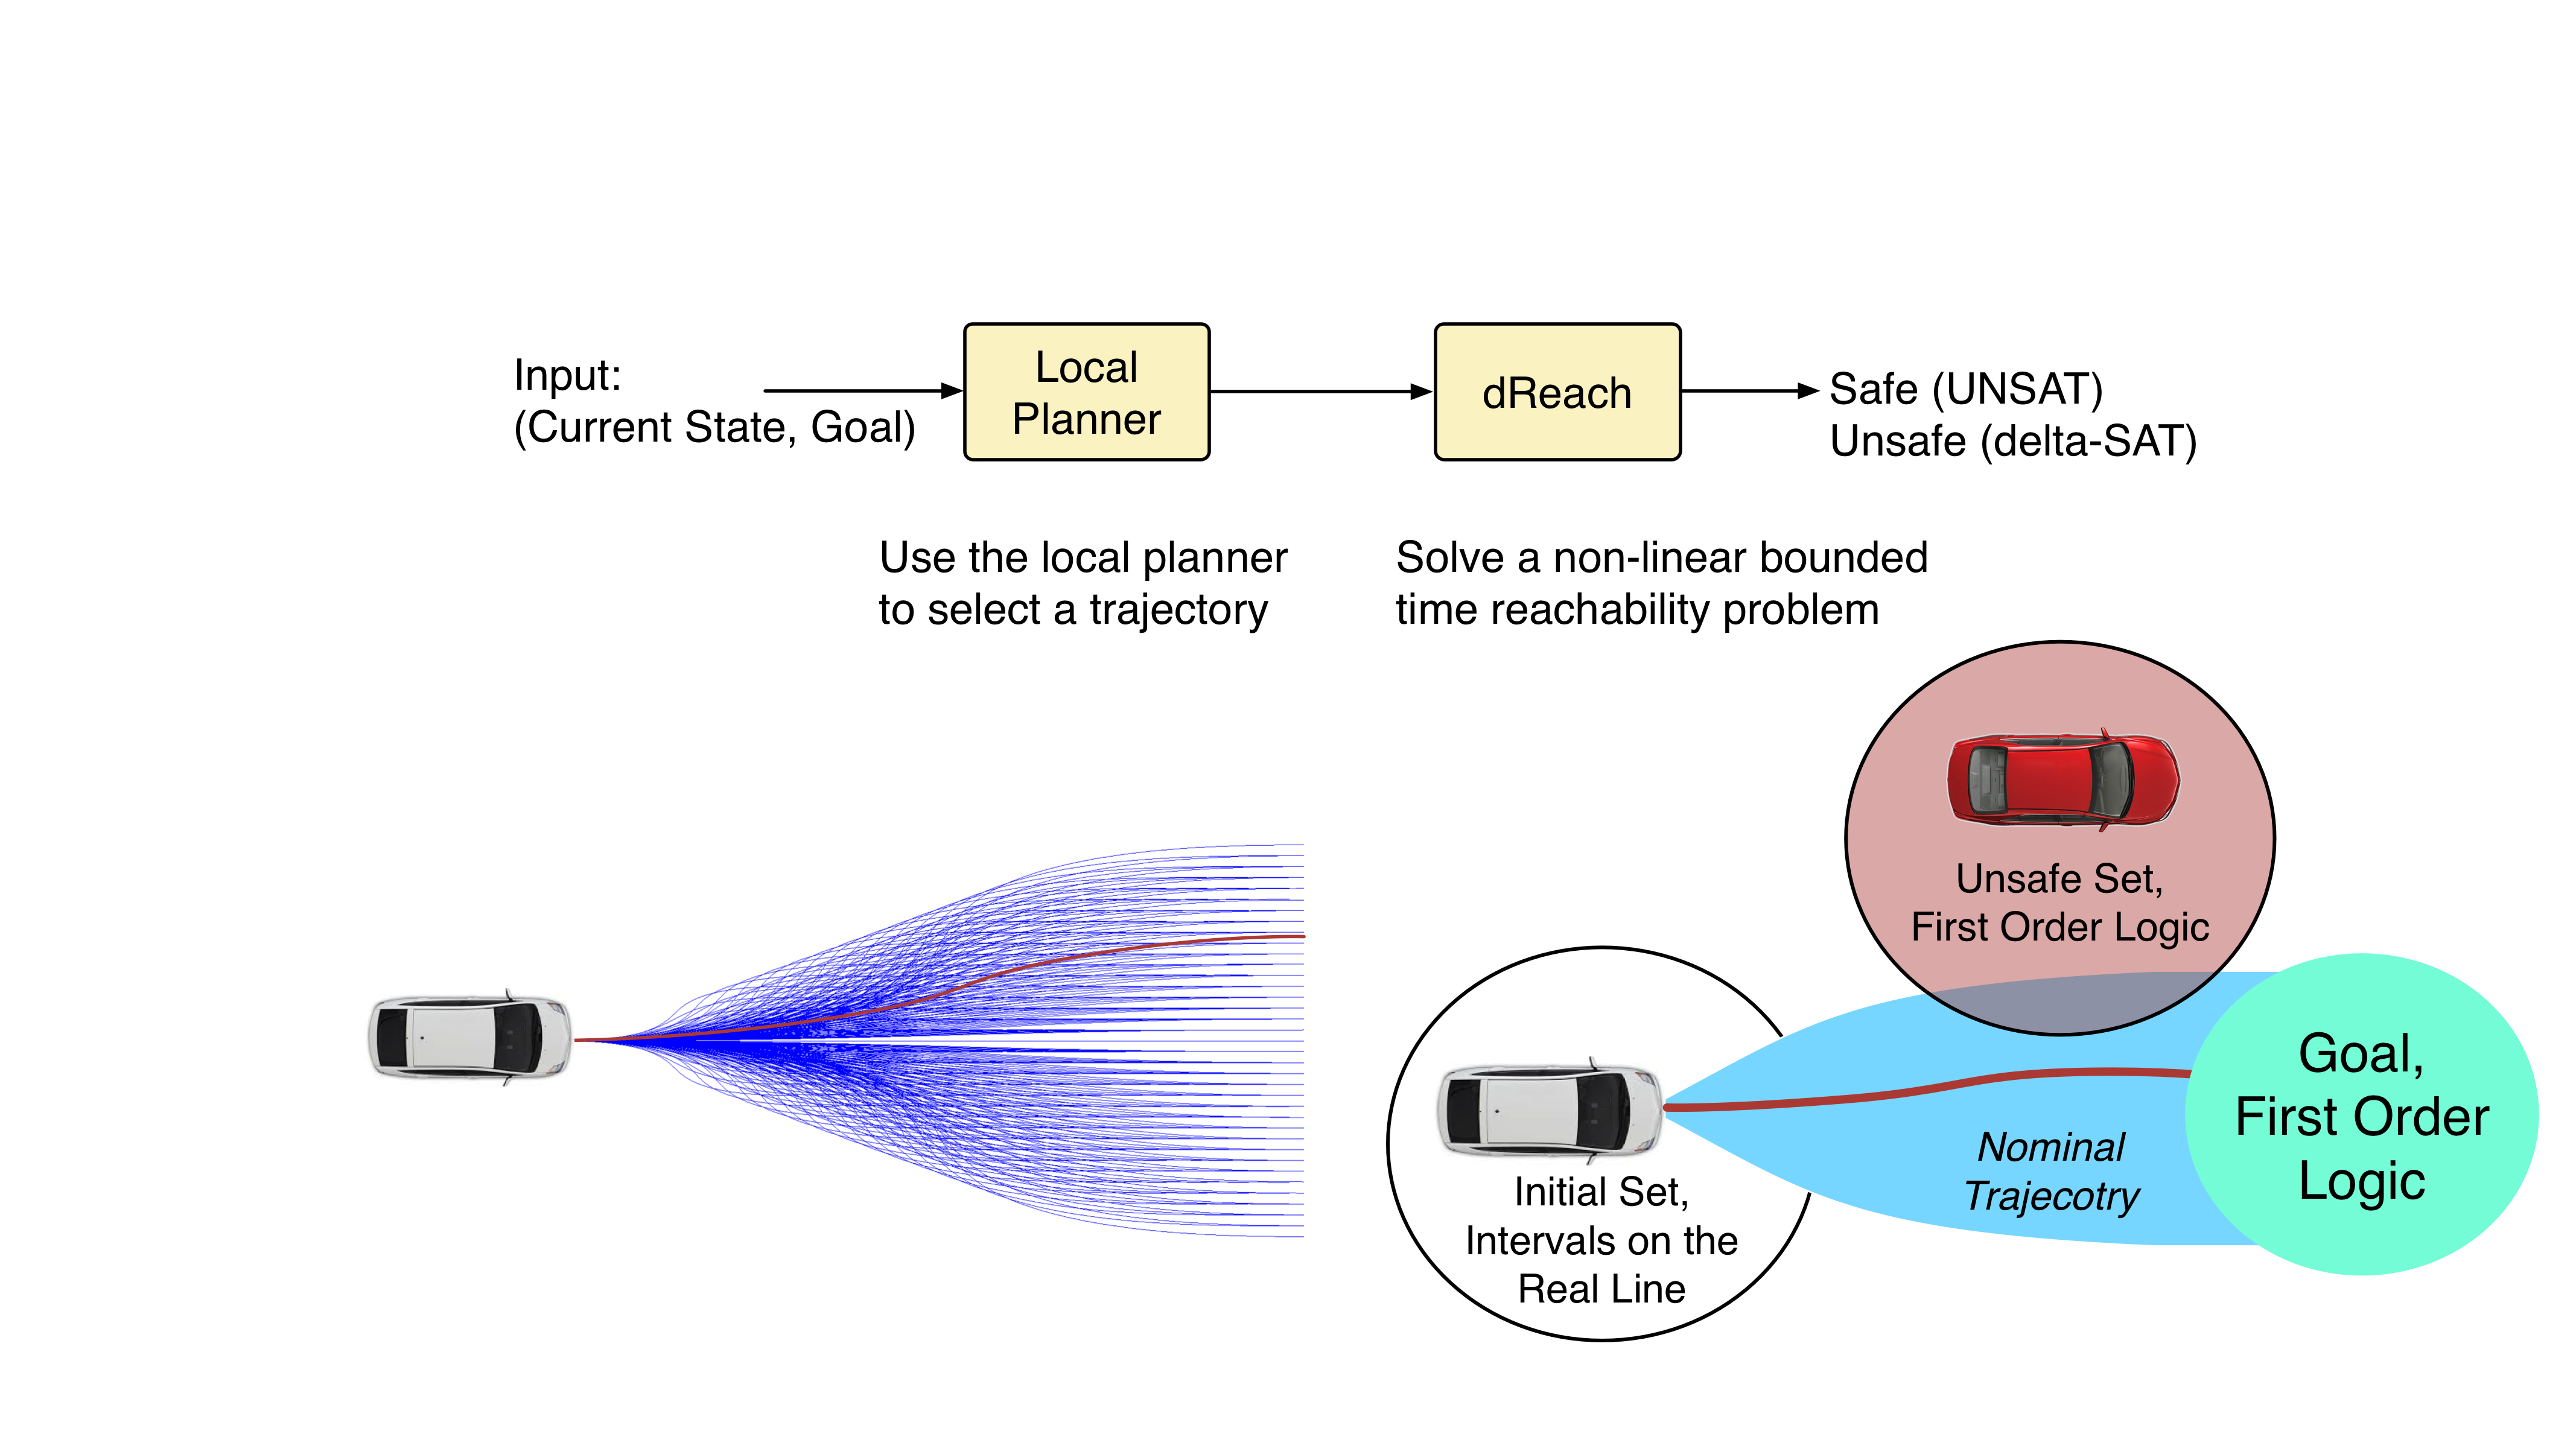
\includegraphics[width=\columnwidth]{figures/tool_single.png}
	\caption{One step in the APEX tool: the local planner generates a trajectory, which is automatically input into the mission description file and verified using dReach}
	\vspace{-10pt}
	\label{fig:apexsingle}
\end{figure}

 \begin{figure*}
 	\centering
 	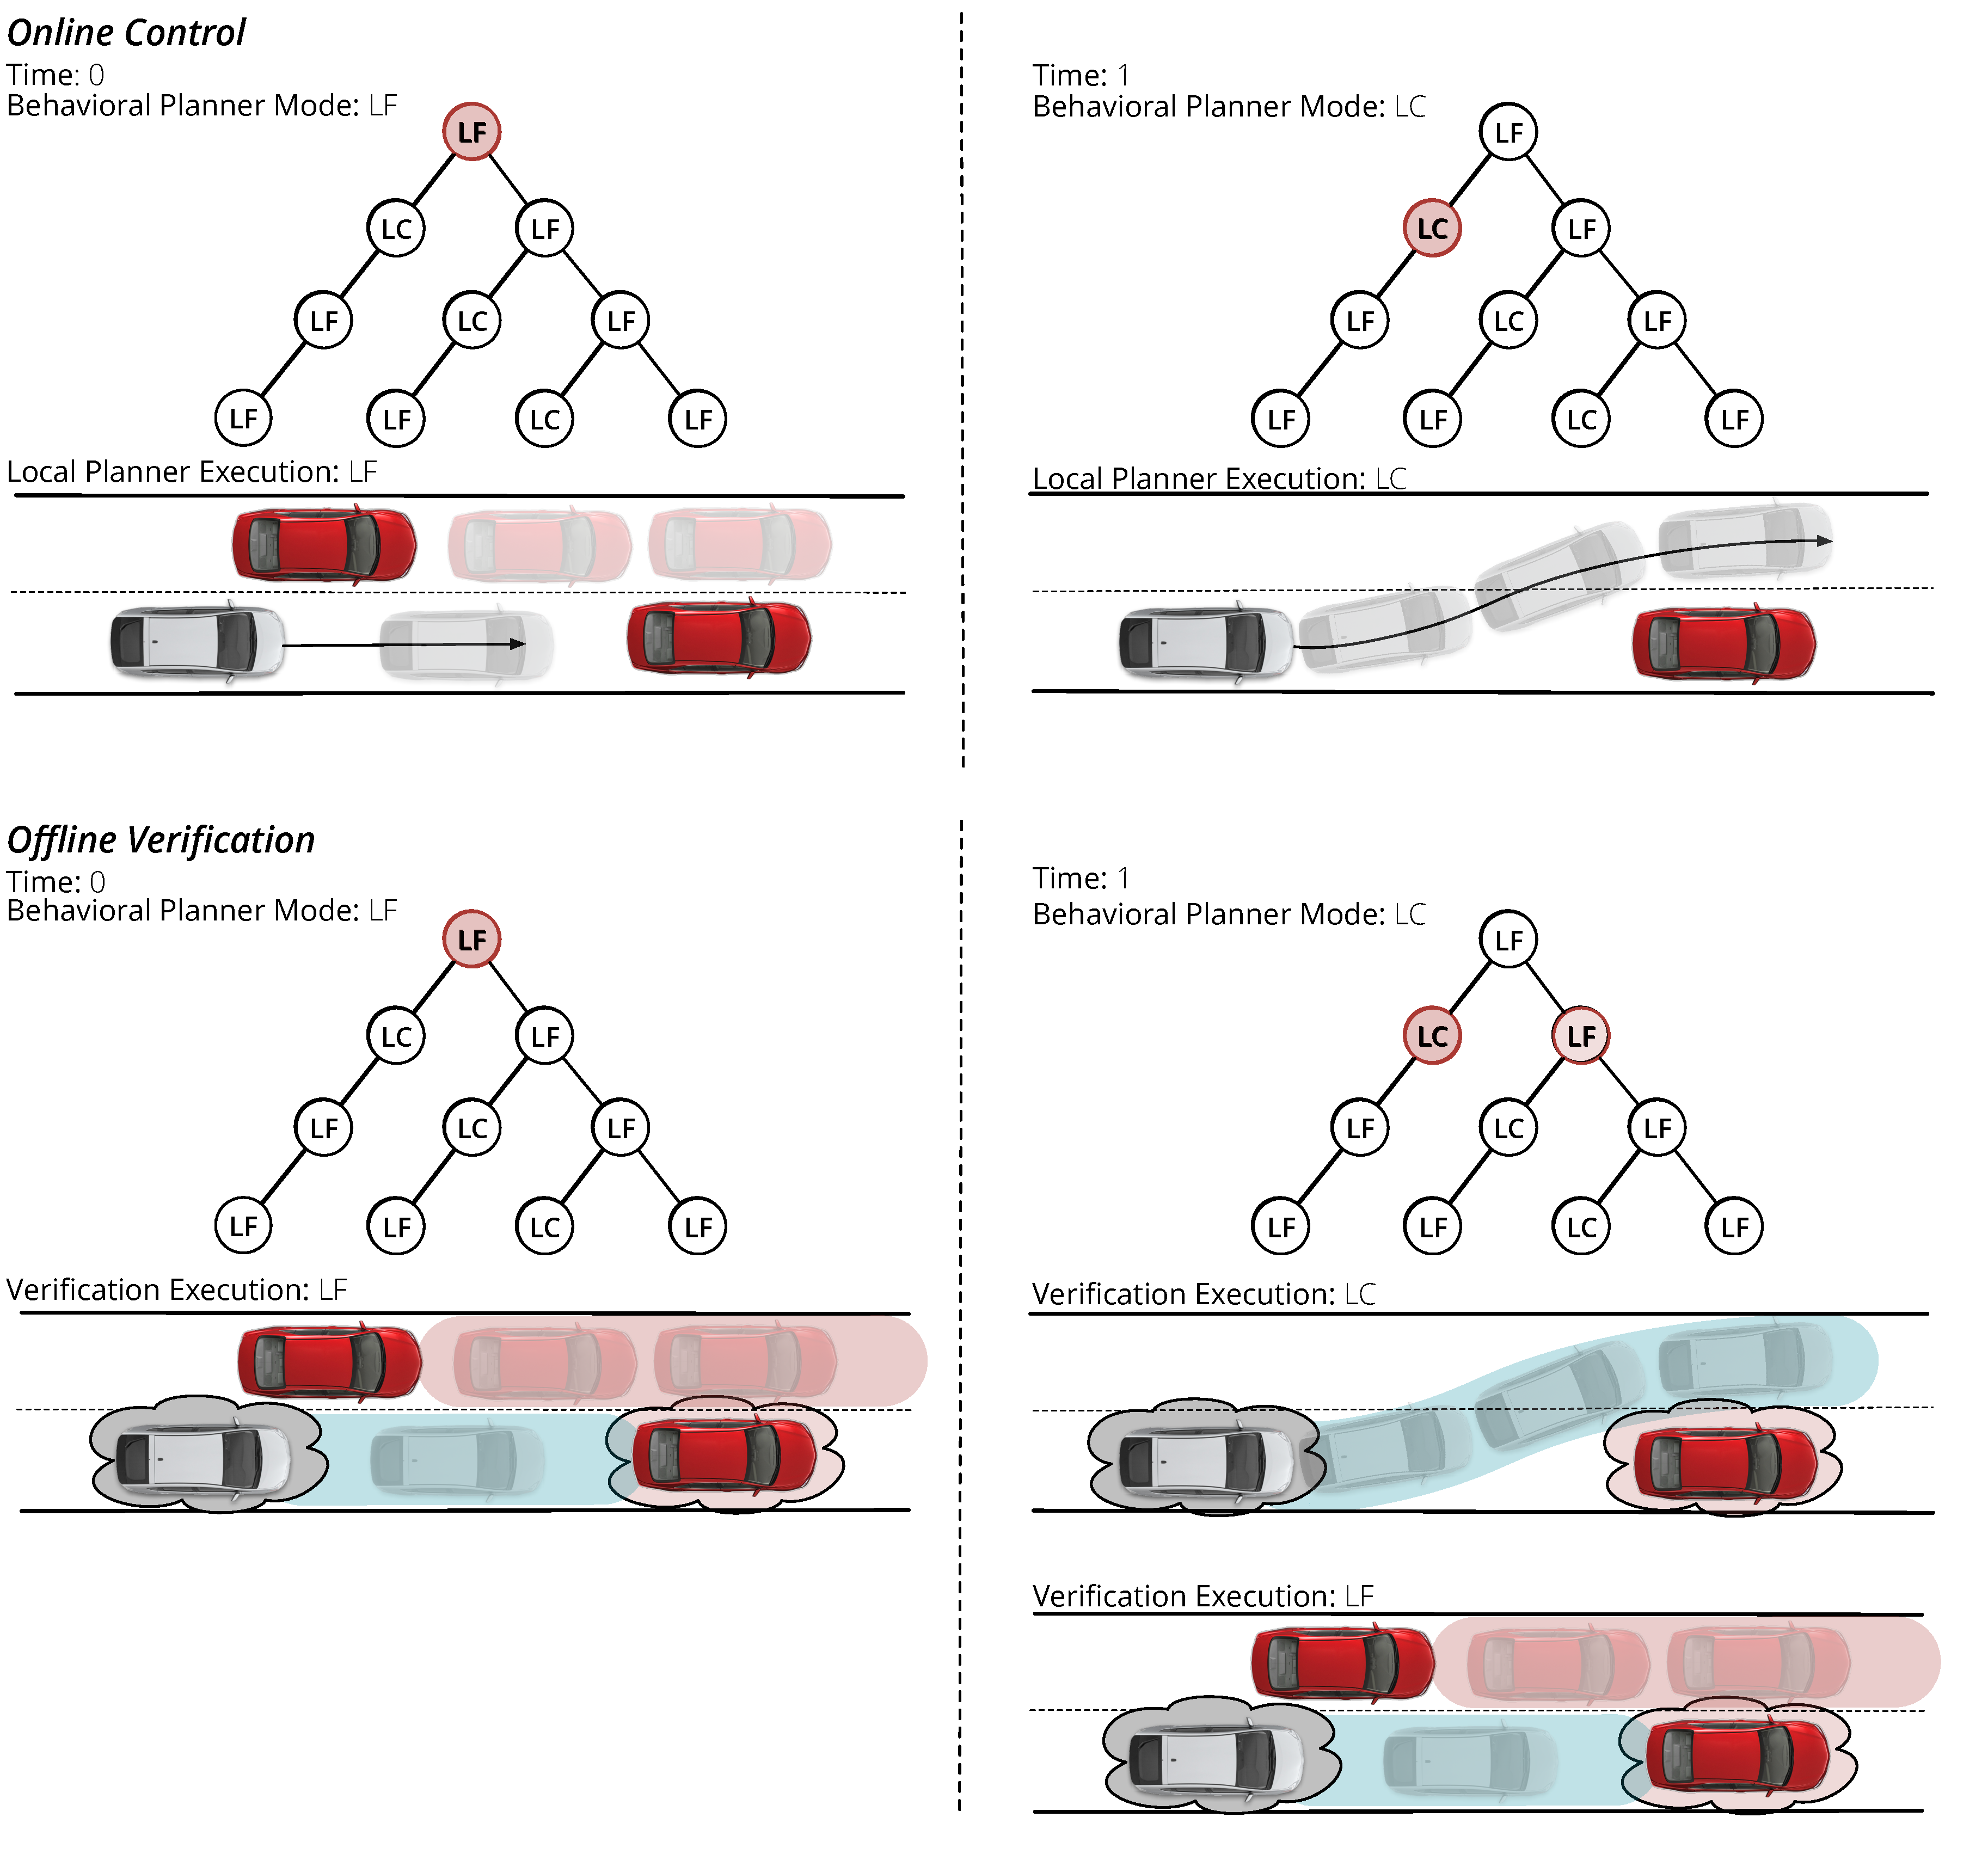
\includegraphics[width=\textwidth]{figures/apex_approach.pdf}
 	\caption{ \small Stages of APEX verification and their correspondence to control execution. Top left: at $t=0$, mode is Lane Follow (LF) and the vehicle follows the current lane. Top right: at $t=1$, mode is Lane Change (LC) and vehicle starts a lane change maneuver. Bottom left: offline, APEX verifies that in mode LF, the vehicle can track the trajectory. Bottom right: offline, APEX verifies both possible executions, a lane change and a lane following.}
	\vspace{-10pt}
 	\label{fig:apex_internals}
 \end{figure*}
APEX answers the following question by re-formulating it as a reachability problem: given some initial uncertainty about the state of the AV, constraints on the configuration of the environment, and a desired behavior of the AV (like mobility goal and traffic laws), is it ever possible for the AV to violate the desired behavior?
Fig. \ref{fig:apexsingle} summarizes a single execution of the verification engine.
For each trajectory selected by the planner (highlighted in red), APEX calls dReach~\cite{gao2014delta}, a reachability analysis tool for nonlinear hybrid systems.
% 
%The APEX approach to formal verification of AVs and ADAS systems seeks to follow plan executions through to the vehicle's actual motion in the environment rather than exploring abstract motion on a grid.

We emphasize that the verification process is \emph{offline} - the vehicle does \emph{not} run APEX while it is driving.
At each decision point encountered by the behavioral planner there may be multiple executions of the verification engine depending on the design of the behavioral planner. Fig. \ref{fig:apex_internals} describes how the execution of the controller online relates to the \emph{offline} verification process. In contrast to the simulation based approach outlined in the introduction, the result of the APEX approach is that we have converted a brute force search over real intervals into a finite series of tractable bounded reachability problems over a finite verification horizon.
% In certain cases we may even deduce infinite time system properties via an investigation of a finite number of reachability problems. 

\subsection{Tool Input}
APEX is a \emph{command line tool} for verification of autonomous vehicle missions written in Python and C++.
The input to the verification process is a \emph{mission definition file}. 
The \emph{mission definition file} defines the sequence of waypoints or road links which the vehicle will traverse in order to achieve a mobility goal. 

The \emph{mission defintion file} describes the following:
\begin{itemize}
	\item \emph{The collection of agents in the scenario}, consisting of the ego vehicle and other cars in the scenario.
	The agents are described via ODEs that describe the evolution of their state with time, and their behavioral planners, which give the next waypoints for each vehicle.
	All agents operate in an ontology specific to the mission, in this case the world model consists of a geometric description of a road network. 
	\item \emph{Set of initial states} for each state variable of every vehicle.
	\item \emph{The constraints that the AV should satisfy}, such as traffic laws and the unsafe conditions that ego vehicle must avoid. These are described in MITL. 
	\item \emph{The goal of the ego vehicle}, also expressed in MITL \cite{alur1996benefits}. 
\end{itemize}

The mission definition file is part of a \emph{mission definition script}.
The latter manages the execution of the behavioral planner and trajectory generator.
Each (state, goal) pair that is encountered on the mission generates at least one trajectory which must be verified. The \emph{mission definition script} automatically updates a \emph{scenario verification instance}. The \emph{scenario verification instance} is a dReach (.drh) file which combines the results of the plan execution with the dynamical model of the vehicle and a low-level trajectory tracking controller. The \emph{agent definition file} contains the dynamical model of the vehicle and the tracking controller is also written using the syntax of dReach, it may be manually edited in order to match mission specific vehicle models. We provide an example of the syntax of the composed \emph{scenario verification instance} in Fig. \ref{fig:scenario_ver}.


Together, the constraints of the environment $\xi$ and ego vehicle goal and constraints $\phi$ constitute the \emph{specification} of the mission.
The mission is a success if every execution of the system (i.e., every simulation) satisfies the specification.
%We stress, however, that we are \emph{not} simulating the scenario. 
%Rather the formal verification approach we use allows us to make assertions about every execution of the system without actually simulating it.

\begin{figure}
	\centering
	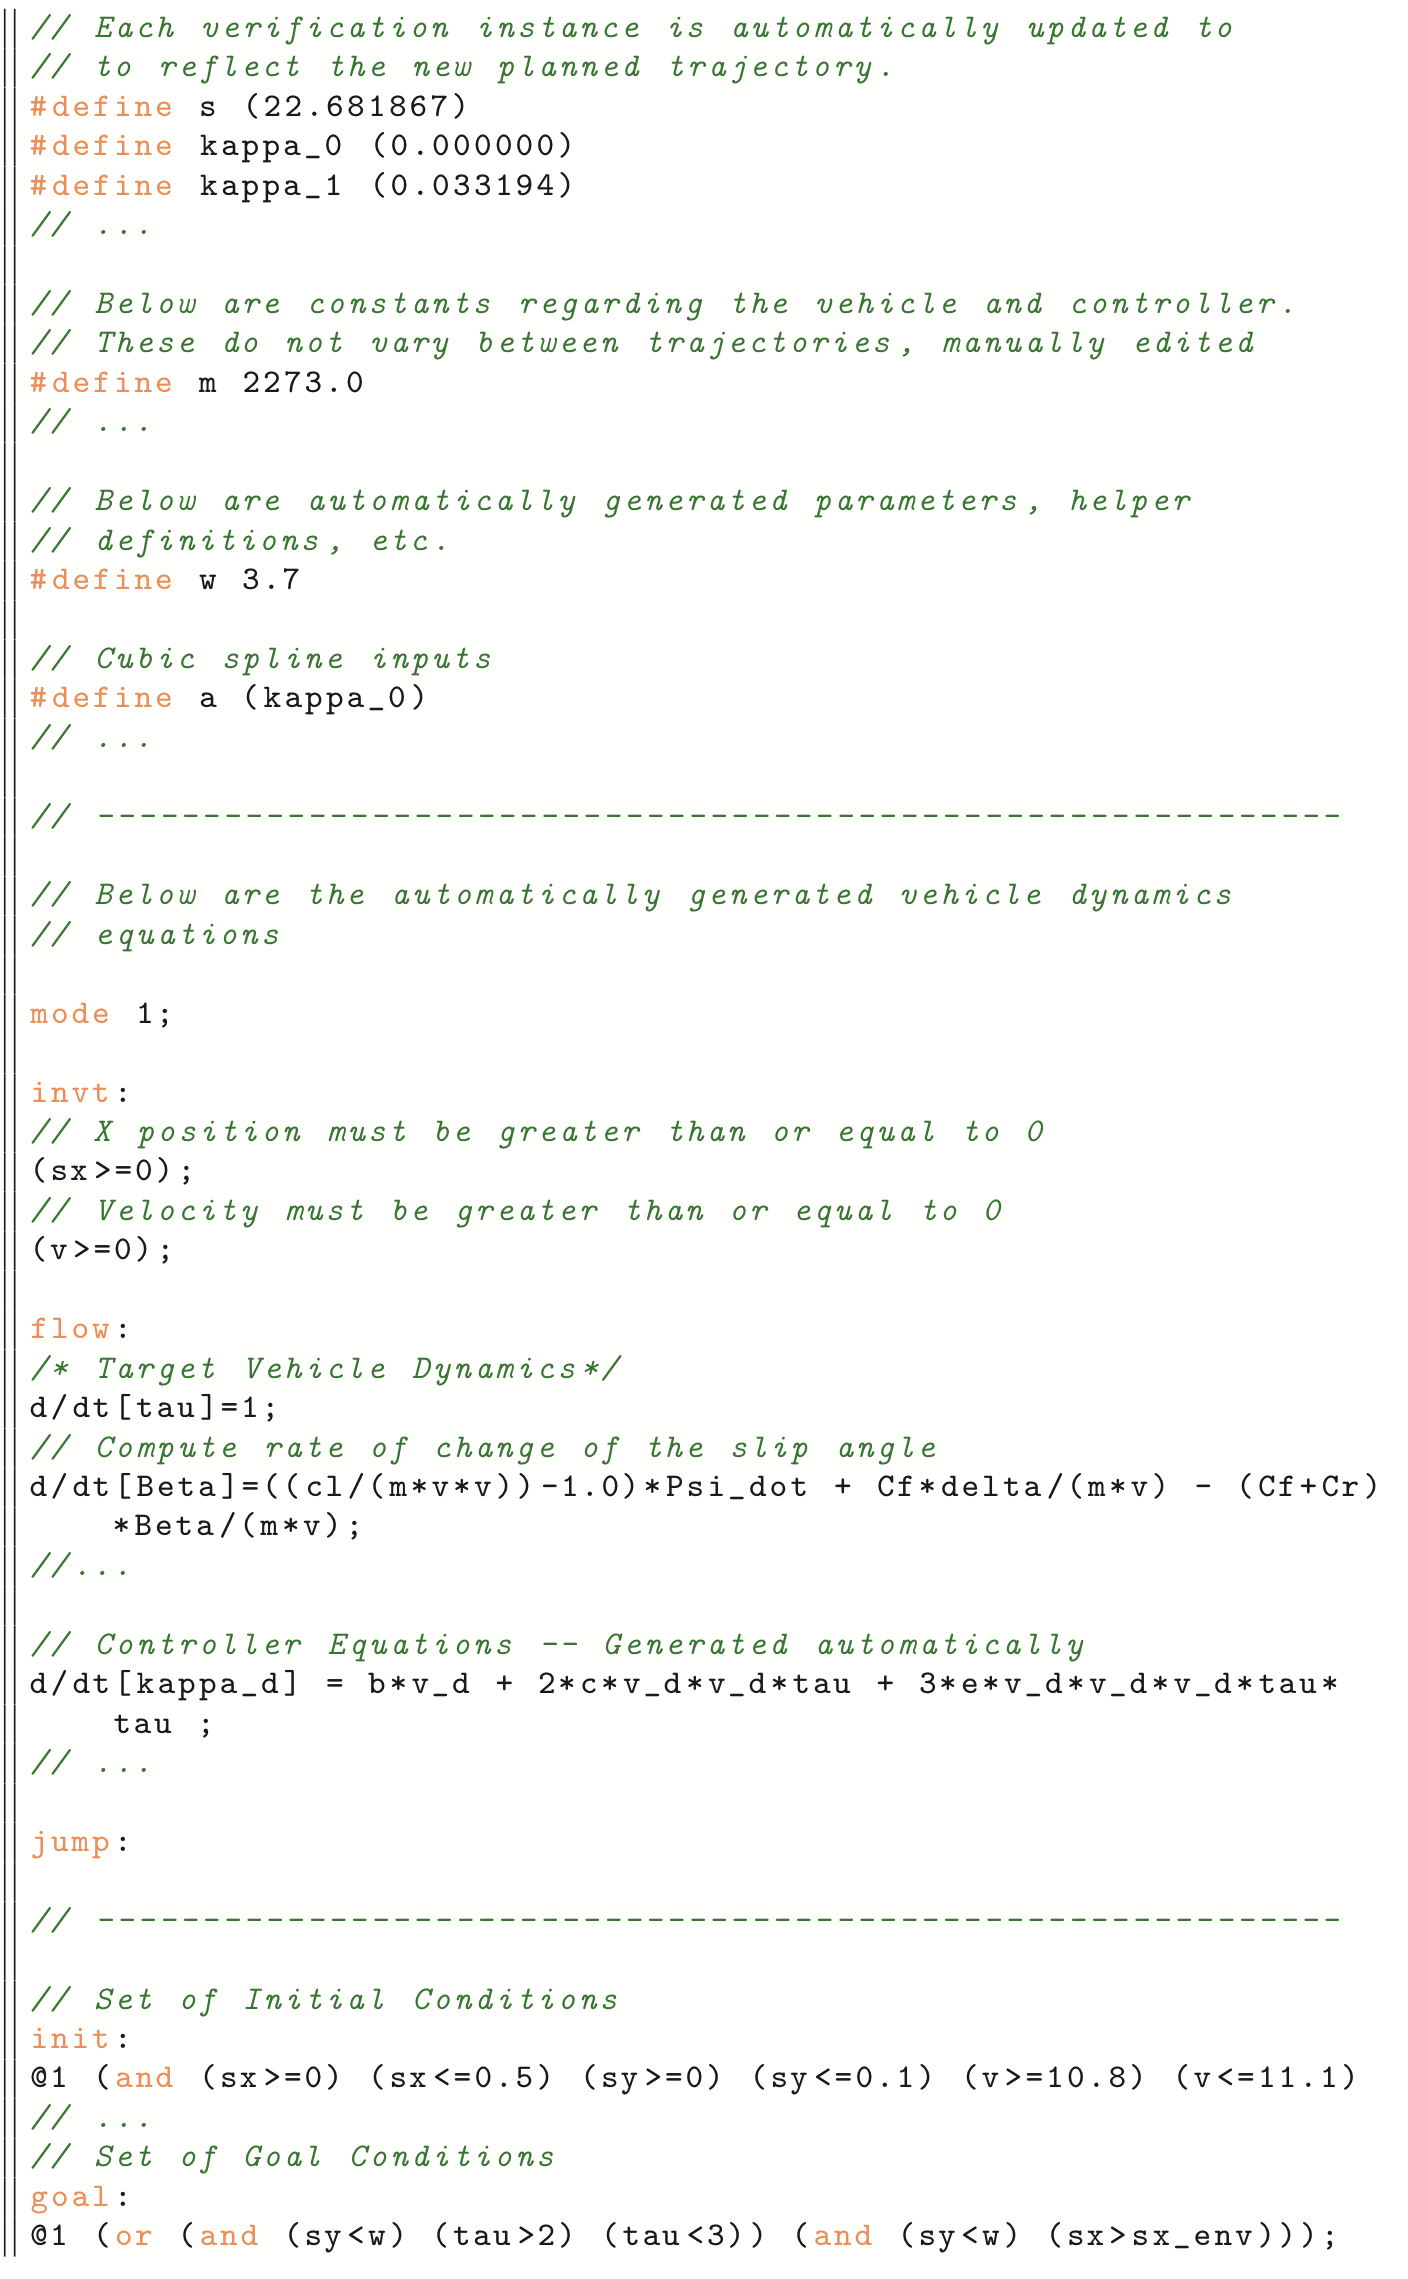
\includegraphics[width=\columnwidth]{figures/code}
	\caption{Scenario verification instance generated by APEX}
	\label{fig:scenario_ver}
\end{figure}

\subsection{Tool Output}
Each \emph{scenario verification instance} can  return either SAFE or $\delta$-UNSAFE. SAFE means that for all possible executions of the system we can not reach an unsafe state.
$\delta$-UNSAFE means that there exists an execution of the system which comes within a $\delta$ of the unsafe region, and possibly enters it. If the system is $\delta$-UNSAFE the tool will return a counter-example describing a tube around a concrete trajectory whose intersection with the unsafe region is not empty. Users of the APEX tool should be aware that selecting too large of a precision value ($\delta$) may result in $\delta$-UNSAFE results which are false positives, but any declaration of SAFE is guaranteed to be correct. 

\section{Simulation and GUI}

\pagebreak
\part{Conclusions}
 \subsection{Future Work: verification, learning, ethics, and control}
 
 %In the literature on robot ethics, it remains arguable whether artificial agents without free
 %will can truly exhibit moral behavior [1]. However, it seems certain that other road users
 %and society will interpret the actions of automated vehicles and the priorities placed by their
 %programmers through an ethical lens. Whether in a court of law or the court of public opinion,
 %the control algorithms that determine the actions of automated vehicles will be subject
 %to close scrutiny after the fact if they result in injury or damage. In a less dramatic, if no
 %less important, manner, the way these vehicles move through the social interactions that
 %define traffic on a daily basis will strongly influence their societal acceptance. This places
 %a considerable responsibility on the programmers of automated vehicles to ensure their
 %control algorithms collectively produce actions that are legally and ethically acceptable to
 %humans.
 %\begin{itemize}
 %	\item Trolley problem
 %	\begin{itemize}
 %		\item Level of semantic detail and embellishment added to such scenarios is unrealistic.
 %		\item The first vehicles to market will simply be programmed with a concept of forward safety.
 %		\item No manufacturer will ever program an autonomous vehicle to swerve into another vehicle. The pretense of such problems is ridiculous.
 %		\item Trolley problem does not have a correct solution, instead we should be asking how can we prove that \emph{trolley problems cannot occur based on decisions made by an autonomous agent}
 %	\end{itemize}
 %\end{itemize}
 
 The likely arrival of learned behaviors and the accompanying cost functions which allow the discrimination between multiple feasible strategies will necessitate careful consideration regarding the quantification of desireable robot behaviors. It is easy to personify the \emph{software agent} which operates an AV; naturally, this leads to the consideration of such an agent's ethical duties. It is not clear whether such software can truly exhibit ethical behavior or rather simply mimic the instructions of the designer. Nevertheless, \quotes{it seems certain that other road users and society will interpret the actions of automated vehicles and the priorities placed by their programmers through an ethical lens} \cite{maurer2015autonomes}. In order to improve the safety, efficacy, and percieved morals of AVs we propose 3 areas of promising future research: 
 \begin{itemize}
 	\item Automatic verification of learned behaviors and cost functions
 	\item Hierarchical property satisfaction and instantiation of temporal logic constraints in a model predictive control framework
 	\item Online verification of behavioral plans \cite{wei2014behavioral} over a range of 5-10 seconds
 \end{itemize}
 
 We have already argued that verification of learned behaviors and cost functions is necessary; we propose that such activities should be fully \emph{automated} in manner similar to static verification of source code. Before an update is released it will be subjected to an ever increasing battery of common verification scenarios. Secondly, we intuit that describing vehicle actions as ethical implies that there exists a ranking function over potential behaviors; if vehicle specifications are described hierarchically we can actually dictate and examine the ethics of a particular AV. For example, it may be desirable that only in a near crash situation the AV disregards the speed limit and lane keeping behaviors in order to avoid an accident. Finally, we propose that such \emph{offline} verification techniques in APEX be reimagined and refactored for short-horizon online verification of all potential vehicle actions. It is likely that initial forays into autonomy may require handoffs between human and machine. Studies show \cite{blanco2013human} that a safe handoff requires 5-8 seconds of preparation. Thus, online verification techniques may be used to discover potential system failures and provide fair warning to the driver. 

\pagebreak
\bibliographystyle{plain}
\bibliography{mok}
 
\end{document}                          % The required last line
